%%%%%%%%%%%%%%%%%%%%%%%%%%%%%%%%%%%%%%%%%%%%%%%%
%
% Strath PhD Thesis Template
%	by Jethro Browell [jethro.browell@strath.ac.uk]
%
%	Guidelines for thesis format, submission and content are found in
%	General and Course Regulations for Graduate and Postgraduate
%	Awards and Degrees, section 20.6.
%
%	Using .eps or .pdf is recomended to prduce high quality figures etc.
%
%	The Strathclyde logo can be found in other formats at www.strath.ac.uk.
%
%%%%%%%%%%%%%%%%%%%%%%%%%%%%%%%%%%%%%%%%%%%%%%%%

\documentclass[a4paper,oneside,11pt]{book}
\setcounter{secnumdepth}{3}
\usepackage{amsbsy}
\usepackage{amsmath}
\usepackage{amsfonts}
\usepackage{graphicx}
\usepackage{multirow}
\usepackage{mathrsfs}
\usepackage{color}
\usepackage[hidelinks]{hyperref}
%\usepackage{cite}
\usepackage{enumitem}
\usepackage{epsfig}
\usepackage{caption}
\usepackage{subcaption}
\usepackage[strict]{changepage}


%\usepackage[utf8]{inputenc}
%\usepackage[T1]{fontenc}
%\usepackage{fontspec}
%\setmainfont{times}
%\usepackage{bookman}


% Page Margins - Strath Requirement
\usepackage[left=4cm,right=2.5cm,top=2cm,bottom=4cm,includehead,includefoot,headheight=15pt]{geometry}

\usepackage[
backend=biber,
bibstyle=numeric,
citestyle=numeric,
minbibnames=3, maxbibnames=3,
]{biblatex}
\addbibresource{thesis_bib.bib}

% Page Headers
\usepackage{fancyhdr}
\fancyhf{}
\renewcommand{\headrulewidth}{0pt} % optional
%\fancyhead[L]{\nouppercase{\leftmark} \hfill Section \nouppercase{\rightmark}}
\fancyhead[L]{\nouppercase{\leftmark}}
\cfoot{\thepage}
\pagestyle{fancy}

% Draft Watermark
%\usepackage[draft=true,allpages=true,fontfamily=cmr,angle=90,scale=0.1,mark={\fboxsep=35pt\fboxrule=0pt\relax\fbox{-- DRAFT -- \today~--}},xcoord=-80,ycoord=-20]{draftmark}

% Line Spacing
%\def\baselinestretch{1.5} 
\usepackage{setspace}
\setstretch{1.5}


% Place UoS Logo on Title Page (this package modifies the "\maketitel" command.)
\usepackage{titling}


%\newcommand*\mycommand[1]{\texttt{\emph{#1}}}

%\newcommand{\comment}[1]{{\bf\textcolor{red}{#1}}}
% \newcommand{\comment}[1]{{{#1}}}


%%%%%%%%%%%%%%%%%%%%%%%%%%%%%%%%%%%%%%%%%%%%%%%%%%%%%%%%%%%%%%%%%%%%%%%%%%%%%%%%
%%%%%%%%%%%%%%%%%%%%%%%%%%%%%%%%%%%%%%%%%%%%%%%%%%%%%%%%%%%%%%%%%%%%%%%%%%%%%%%%
%%%%%%%%%%%%%%%%%%%%%%%%%%%%%%%%%%%%%%%%%%%%%%%%%%%%%%%%%%%%%%%%%%%%%%%%%%%%%%%%
\begin{document}
	
\setcounter{chapter}{5}
\chapter{Effects of localised shearing on crystal growth and nucleation}
As outlined in Chapter 1, part of the projects aim is to investigate 
the possibility of using optical tweezing to induce nucleation by 
generating fluid flow within a supersaturated solution. The intent 
of which would be twofold: Firstly to have a repeatable means of 
inducing nucleation under different solution conditions. And secondly, 
to understand the influence of shearing on nucleation at a micro 
level as compared to results in bulk fluid. 

It has been shown that for macro-scale systems, the likelihood of 
nucleation increases to a maximum value under increased shearing 
\cite{Debuysschere2023, Mura2016}. Mura and Zaccone developed a 
theoretical framework to describe how the a newly formed nucleus 
experiences two additional growth factors when placed in a moving 
fluid. Firstly, due to increased molecular transport of solute 
molecules the nucleation rate is enhanced in low to moderate fluid 
flows. But in addition, due to shear flow the crystal surface 
undergoes deformation which suppresses the nucleation rate 
undergoing faster fluid flow \cite{Mura2016}. Experimental results 
with glycine solution support this theory; Debuysschere \textit{et 
al} demonstrated that the nucleation rate of supersaturated glycine 
was enhanced up until $\dot{\gamma}\approx3000\ s^{-1}$ 
\cite{Debuysschere2023}. After which the nucleation rate began to 
decrease but was still greater compared to the case where fluid 
flow was minimal.

Optical tweezers can been used to rotate a whole host of microscopic 
objects, with the fastest reported results exceeding $1000\ Hz$ in 
heavy water \cite{Arita2016}. If such a micro-rotor was suspended in
a supersaturated solution the fluid flow around it could be fast enough
that the nucleation rate is locally enhanced. We focused on two 
primary candidates for rotation, Vaterite and 
4-Heptyl-4-biphenylcarbonitrile (7CB). The former being a polymorph of 
calcium carbonate and the latter an example of nematic liquid crystals, 
both of which have been used repeatedly in previous micro-rotor research
\cite{Saito2022, Arita2016, Parkin2009}. In addition, we also consider 
the application of using techniques beam steering to generate fluid 
flow by trapping silica micro-beads. In this instance the fluid flow is 
generated not due to the transfer of angular momentum, but due to 
shearing caused by a moving sphere through stagnant fluid.

To begin with, the discussion of the necessary optical equipment is 
covered, drawing attention to specialised components and techniques 
that are not standard in optical trapping set ups.
%%%%%%%%%%%%%%%%%%%%%%%%%%%%%%%%%%%%%%%%%%%%%%%%%%%%%%%%%%%%%%%%%%%%%%%%%%%%%%%%
%%%%%%%%%%%%%%%%%%%%%%%%%%%%%%%%%%%%%%%%%%%%%%%%%%%%%%%%%%%%%%%%%%%%%%%%%%%%%%%% 
\section{Optical Tweezer Equipment}
In general, all optical tweezers require a laser driver, a focusing 
microscope objectives, a position controller, and position detector 
\cite{Gieseler2020}. The laser used for this project was a $1064\ 
nm$ near infrared laser - provided by CNI Lasers – that was focused 
by a Nikon 100x oil immersion lens. The choice of an oil immersion 
lens is important as the optical oil used prevents a loss of focus 
when used on a glass cover slip. Now, experimental work has shown 
that the trapping efficiency increases with beam diameter up until 
it exceeds $\frac{2}{3}D_{obj}$ \cite{kim2003dependence} where 
$D_{obj}$ is the diameter of the objective aperture. To expand the 
beam front we utilise a Galilean beam expansion arrangement 
(indicated by $f_1$, and $f_2$ in Fig.~\ref{fig:setup}) as recommended 
for high power laser applications. In our initial experiments the 
beam expansion provides a $4\times$ magnification. Whereas in later 
experiments we utilised a galvano-mirror the beam expansion is 
$3\times$ and then the 4f correlator (see \ref{sec:4f_correlation})
provides a further $1.25\times$ magnification (using $f_3$ and $f_4$) 
- the magnification is given by.
\begin{align}
	\frac{D_2}{D_1} = \frac{f_2}{f_1}
\end{align}

It should be noted that the galvano-mirror requires the use of a 
Keplerian beam expansion arrangement which reduces the transmitted 
laser power due to localised heating of the air. Afterwards the 
laser is passed through a dichroic mirror that separates incoming 
infrared and visible light, this is to prevent the laser from 
damaging the CCD camera used for imaging the trapping plane. The 
laser is then focused to a diffraction limited spot by the objective. 
Utilizing a high numerical aperture objective enhances the gradient 
force at the focal point; the trade-off being that the for higher NA 
objectives the trapping depth is reduced due to spherical aberrations. 
While it is possible to increase the trapping depth \cite{Reihani2006} 
by adjusting the objective's tube length this approach is incompatible 
with our trapping arrangement. A 0.25 NA condenser objective refocuses 
the scattered laser light and also provide an aperture for an imaging 
LED to illuminate the focal plane. Samples are loaded onto a piezo 
driven table to that is inserted between the trapping and condensing 
objectives; the piezo drivers allow for sub-micron control of the 
beam focus position to a degree as small as a 10 nm. To detect and 
monitor the position of a trapped particle a quadrant photo diode 
(QPD) was utilised. 
\begin{figure}[h!]
	\centering
	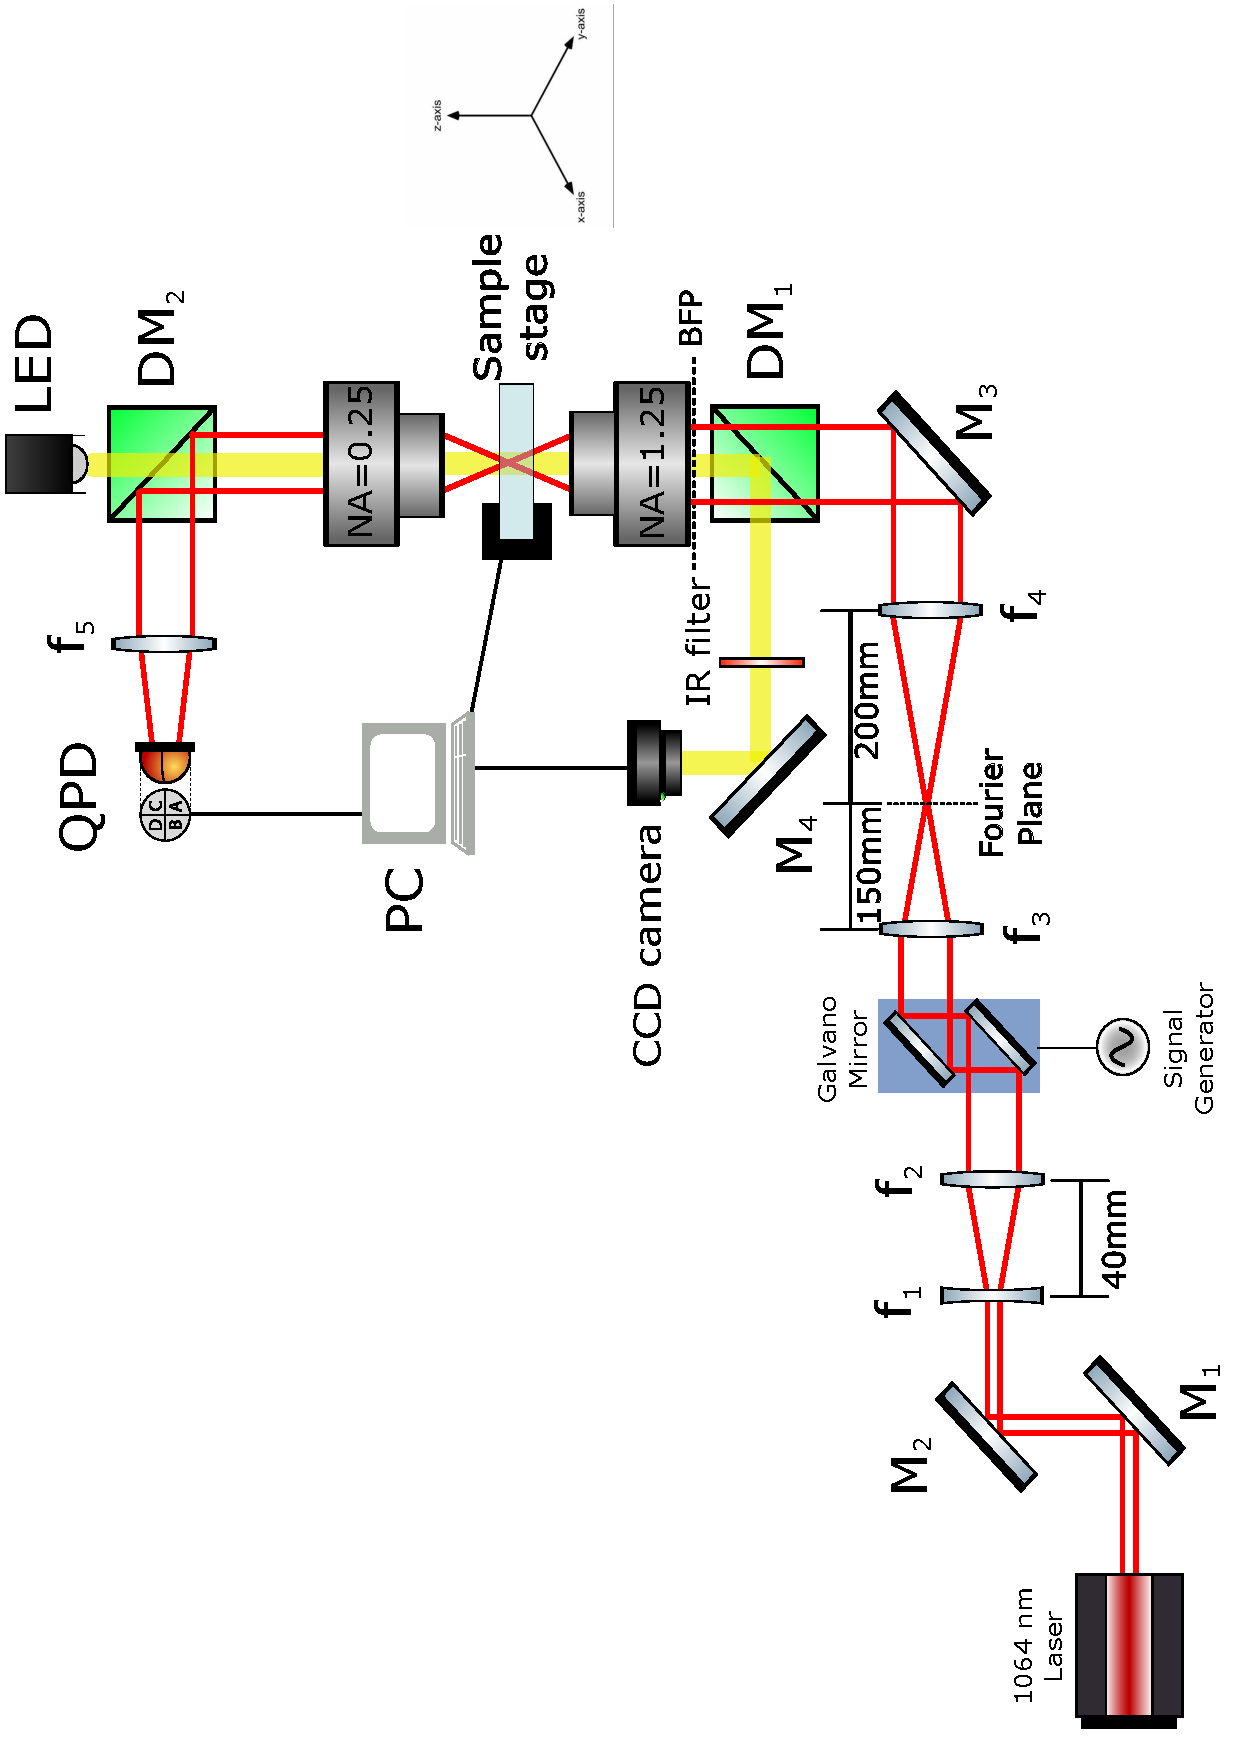
\includegraphics[height=\linewidth, angle=270]{tweezer_setup.pdf}
	\caption{Optical tweezer set up used for the majority of the PhD. 
		The focal lengths of $f_1$, $f_2$, $f_3$, \& $f_4$ are $-20\ mm$, 
		$60\ mm$, $150\ mm$, \& $200\ mm$ respectively [M = mirrors,
		DM = dichroic mirrors, f = focal lenses]. Diagram not 
		drawn to scale.}
	\label{fig:setup}
\end{figure}

%%%%%%%%%%%%%%%%%%%%%%%%%%%%%%%%%%%%%%%%%%%%%%%%%%%%%%%%%%%%%%%%%%%%%%%%%%%%%%%%
\subsection{Position detection}
\label{sec:position_detection}
In order to accurately capture the dynamics of a trapped particle, a 
position detection system is required. There are 3 possible methods 
of position detection: video-analysis, lateral-effect position sensing, 
and photodiodes. 

Video analysis is ideally suited for multiple traps or situations where 
precision is not the top priority. Whereas lateral-effect and photodiode 
position detection are two examples of back-focal plane interferometry, 
where the interference pattern produced by the target particle is 
extrapolated to determine its position. In order for video analysis to 
match the accuracy of back-focal plane interferometry methods requires 
the camera's frame rate to exceed $1\ kHz$ which can be difficult to 
achieve while maintaining a decent resolution \cite{Gibson2008}. In 
comparison off the shelf back-focal plane detectors can achieve temporal 
resolutions anywhere from $10-100\ kHz$ \cite{BergSoerensen2004}. 
 
A lateral-effect sensor has a similar output but works using a the 
entire sensor as a single cell analogous to the focal plane of the 
trapping beam. The four corners of the sensor act as anodes connected 
to a base plate cathode, as the beam moves across the surface of the 
detector each anode will experience a different photocurrent depending 
on how close the centre of the interference pattern is to each anode. 
The advantage of a lateral effect detector is that the linear regime 
is much larger than a QPD making it much better for monitoring the 
position of a trapped particle. However, Lateral-effect sensors are 
often limited in their spacial resolution due to high signal-to-noise 
ratios, requiring a high intensity of light on the sensor in order to 
get a clean signal. As a result, most optical force measurements are 
conducted using a QPD as opposed to a lateral-effect sensor, as often 
the displacement is small enough that the signal-displacement curve 
can be considered linear.
\begin{figure}[h!]
	\centering
	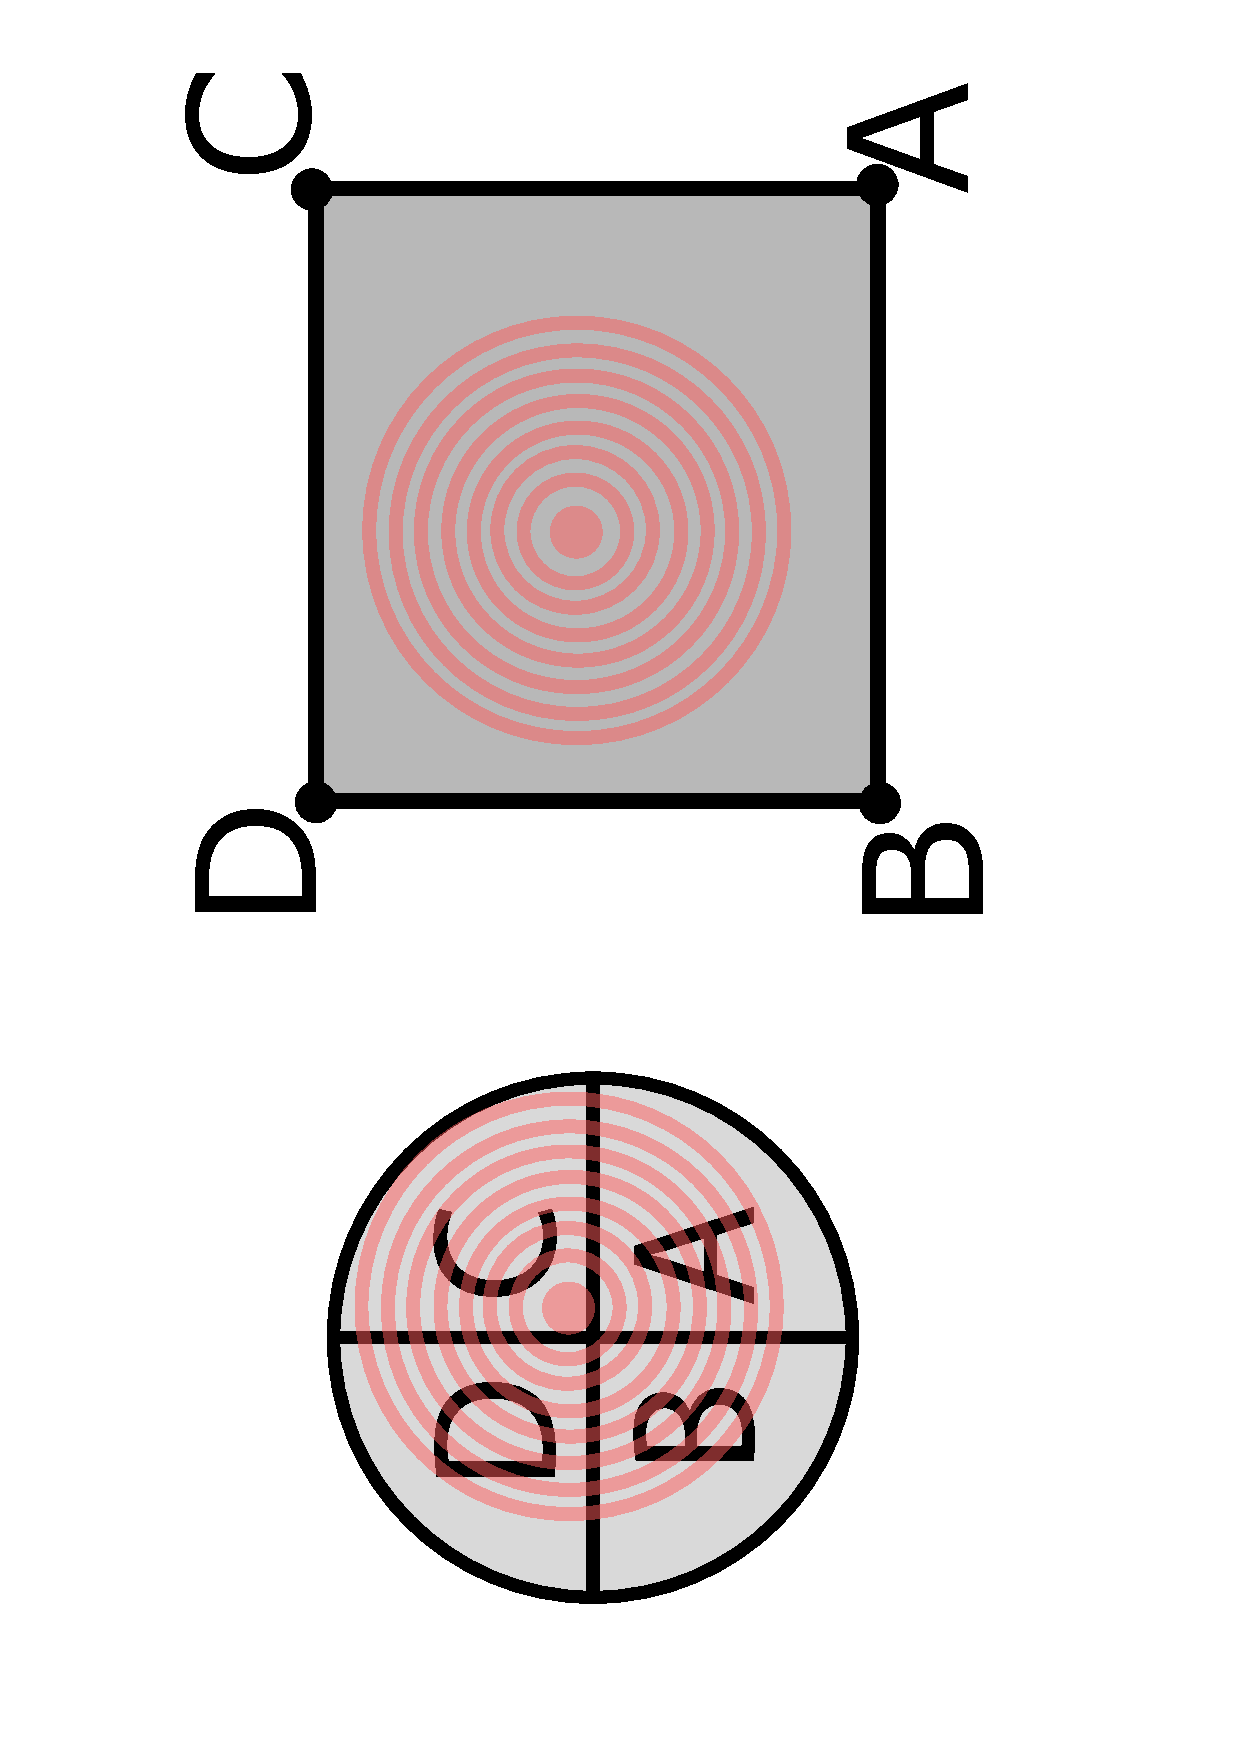
\includegraphics[height=\linewidth, angle=270]{QPD_Lateral_effect.pdf}
	\caption{Comparison between QPD and Lateral effect photodiodes.
	The four quadrants of a QPD (left) experience different photocurrents
	based on the total intensity of light incident on each section 
	(labelled A, B, C, D). 
	Whereas a Lateral effect sensor (right) uses the resistive properties
	of the photodiode surface to vary the create different photocurrents 
	passing through the anodes A, B, C, and D.}
\end{figure}

A quadrant photo diode (QPD) is a frequently used position detection 
system for optical tweezers due to their high sampling rate, high 
degree of precision, and ease of set up. The QPD is constructed of 
four photo diodes assembled in a quadrant formation, when a particle 
is trapped the interference pattern produced is focused onto the QPD, 
with the maximum intensity mapping to the particle's centre of mass. 
By summing the voltages of the horizontal and vertical quadrants together 
the particle's centre of mass is tracked in the x-y plane. Axial 
displacement can be estimated by observing the change in the total 
voltage of the QPD. The outputted signal gives an indication of the 
particle's relative displacement from the beam focus, but in order to 
convert the signal to distance units the trap needs to be calibrated 
(assuming a linear response curve).

%%%%%%%%%%%%%%%%%%%%%%%%%%%%%%%%%%%%%%%%%%%%%%%%%%%%%%%%%%%%%%%%%%%%%%%%%%%%%%%
\subsection{Fourier Optics and 4f correlators}
\label{sec:4f_correlation}
As shown in \ref{fig:setup}, after the Galvano mirror there are a pair
of focal lenses ($f_3$ and $f_4$) that do not seem to serve a clear
purpose. These are in fact crucial for the operation of the Galvano, the
pair of them can be more accurately called a 4f correlator. 

A 4f correlator is an example of Fourier optics in practice, understanding
that a focused lens takes a Fourier transform of the light profile. 
Consider a laser with a circular Gaussian profile, if you were to place 
a detector there you would pick up the intensity as a function of its 
position within the beam. If however you focused the light into a single 
point (using a +ve focal lens) you are actually seeing a measurement of 
the phase of your laser with position, in which you would see a diffraction
limited spot ($d = \lambda/2nsin(\theta)$), indicating that the laser is 
collimated. In imaging systems, a series of focal lenses can be used to 
filter out unwanted scattering from an image (or in an inverse case 
differentiate between different images), the placement of each lens is 
shown via fig.~\ref{fig:signal_generator}.
\begin{figure}[h!]
	\centering
	\begin{subfigure}{0.475\linewidth}
		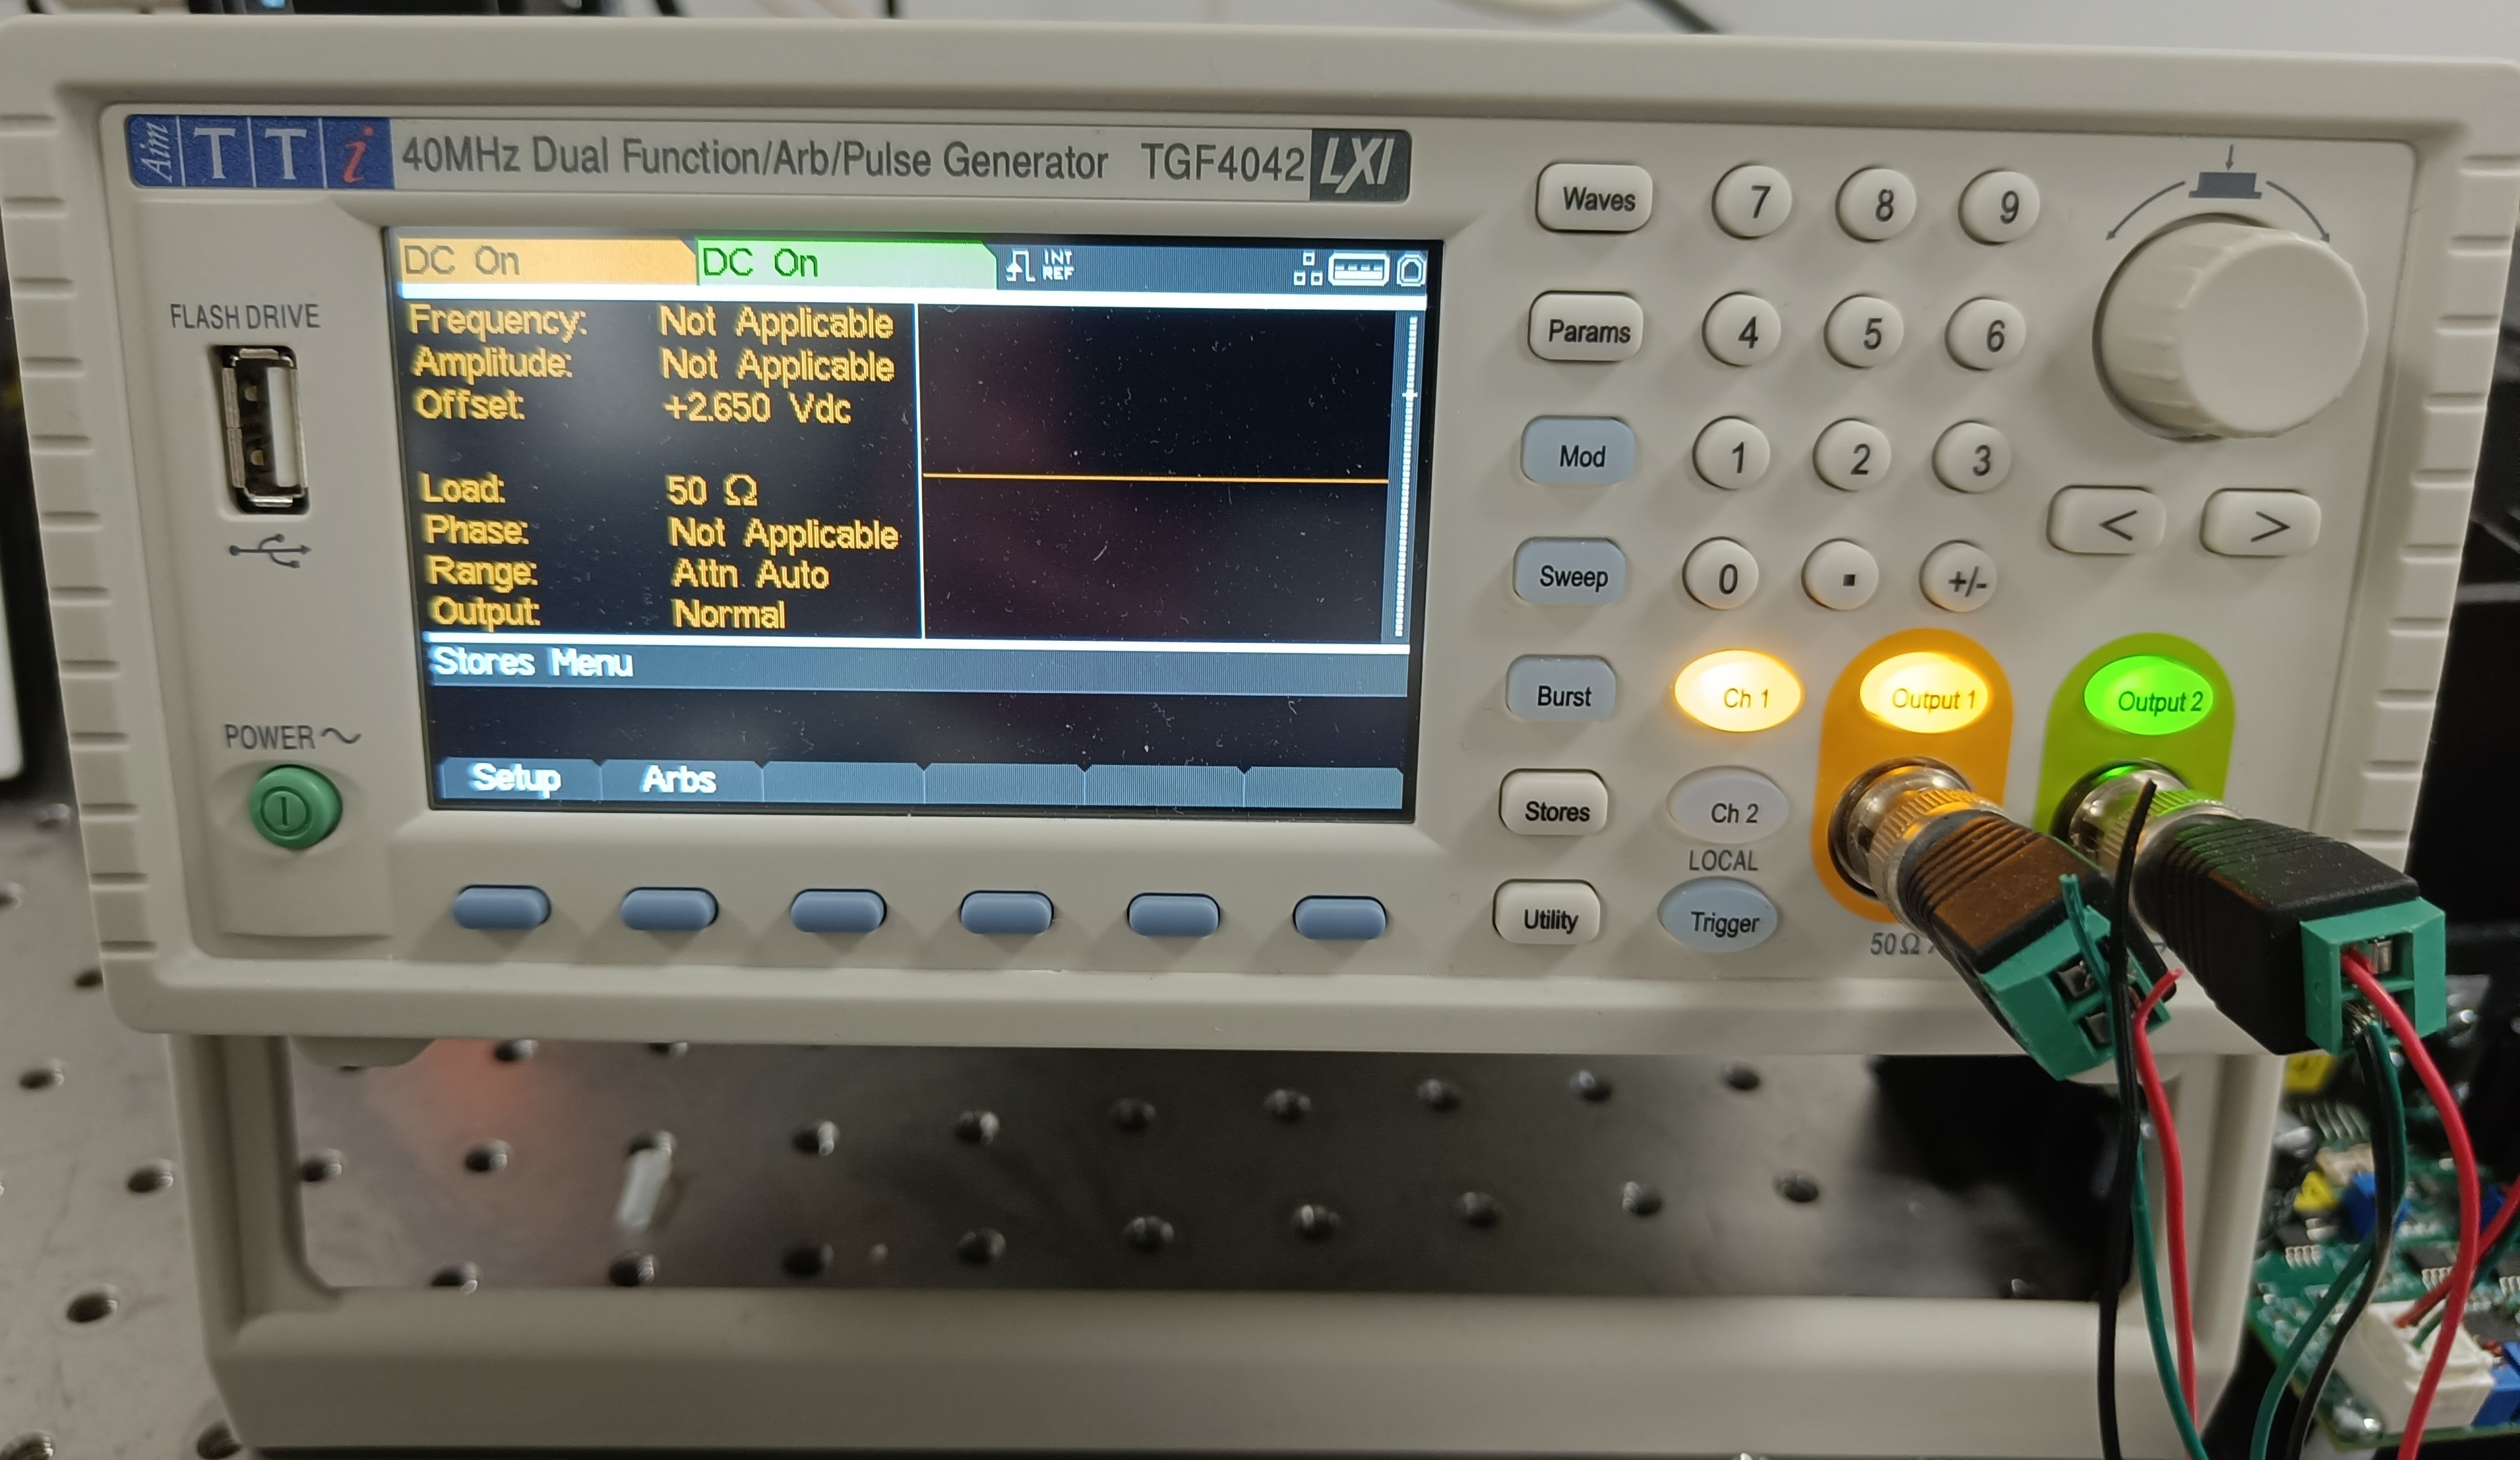
\includegraphics[width=\linewidth]{signal_generator.jpg}
		\caption{}
	\end{subfigure}
	\begin{subfigure}{0.475\linewidth}
		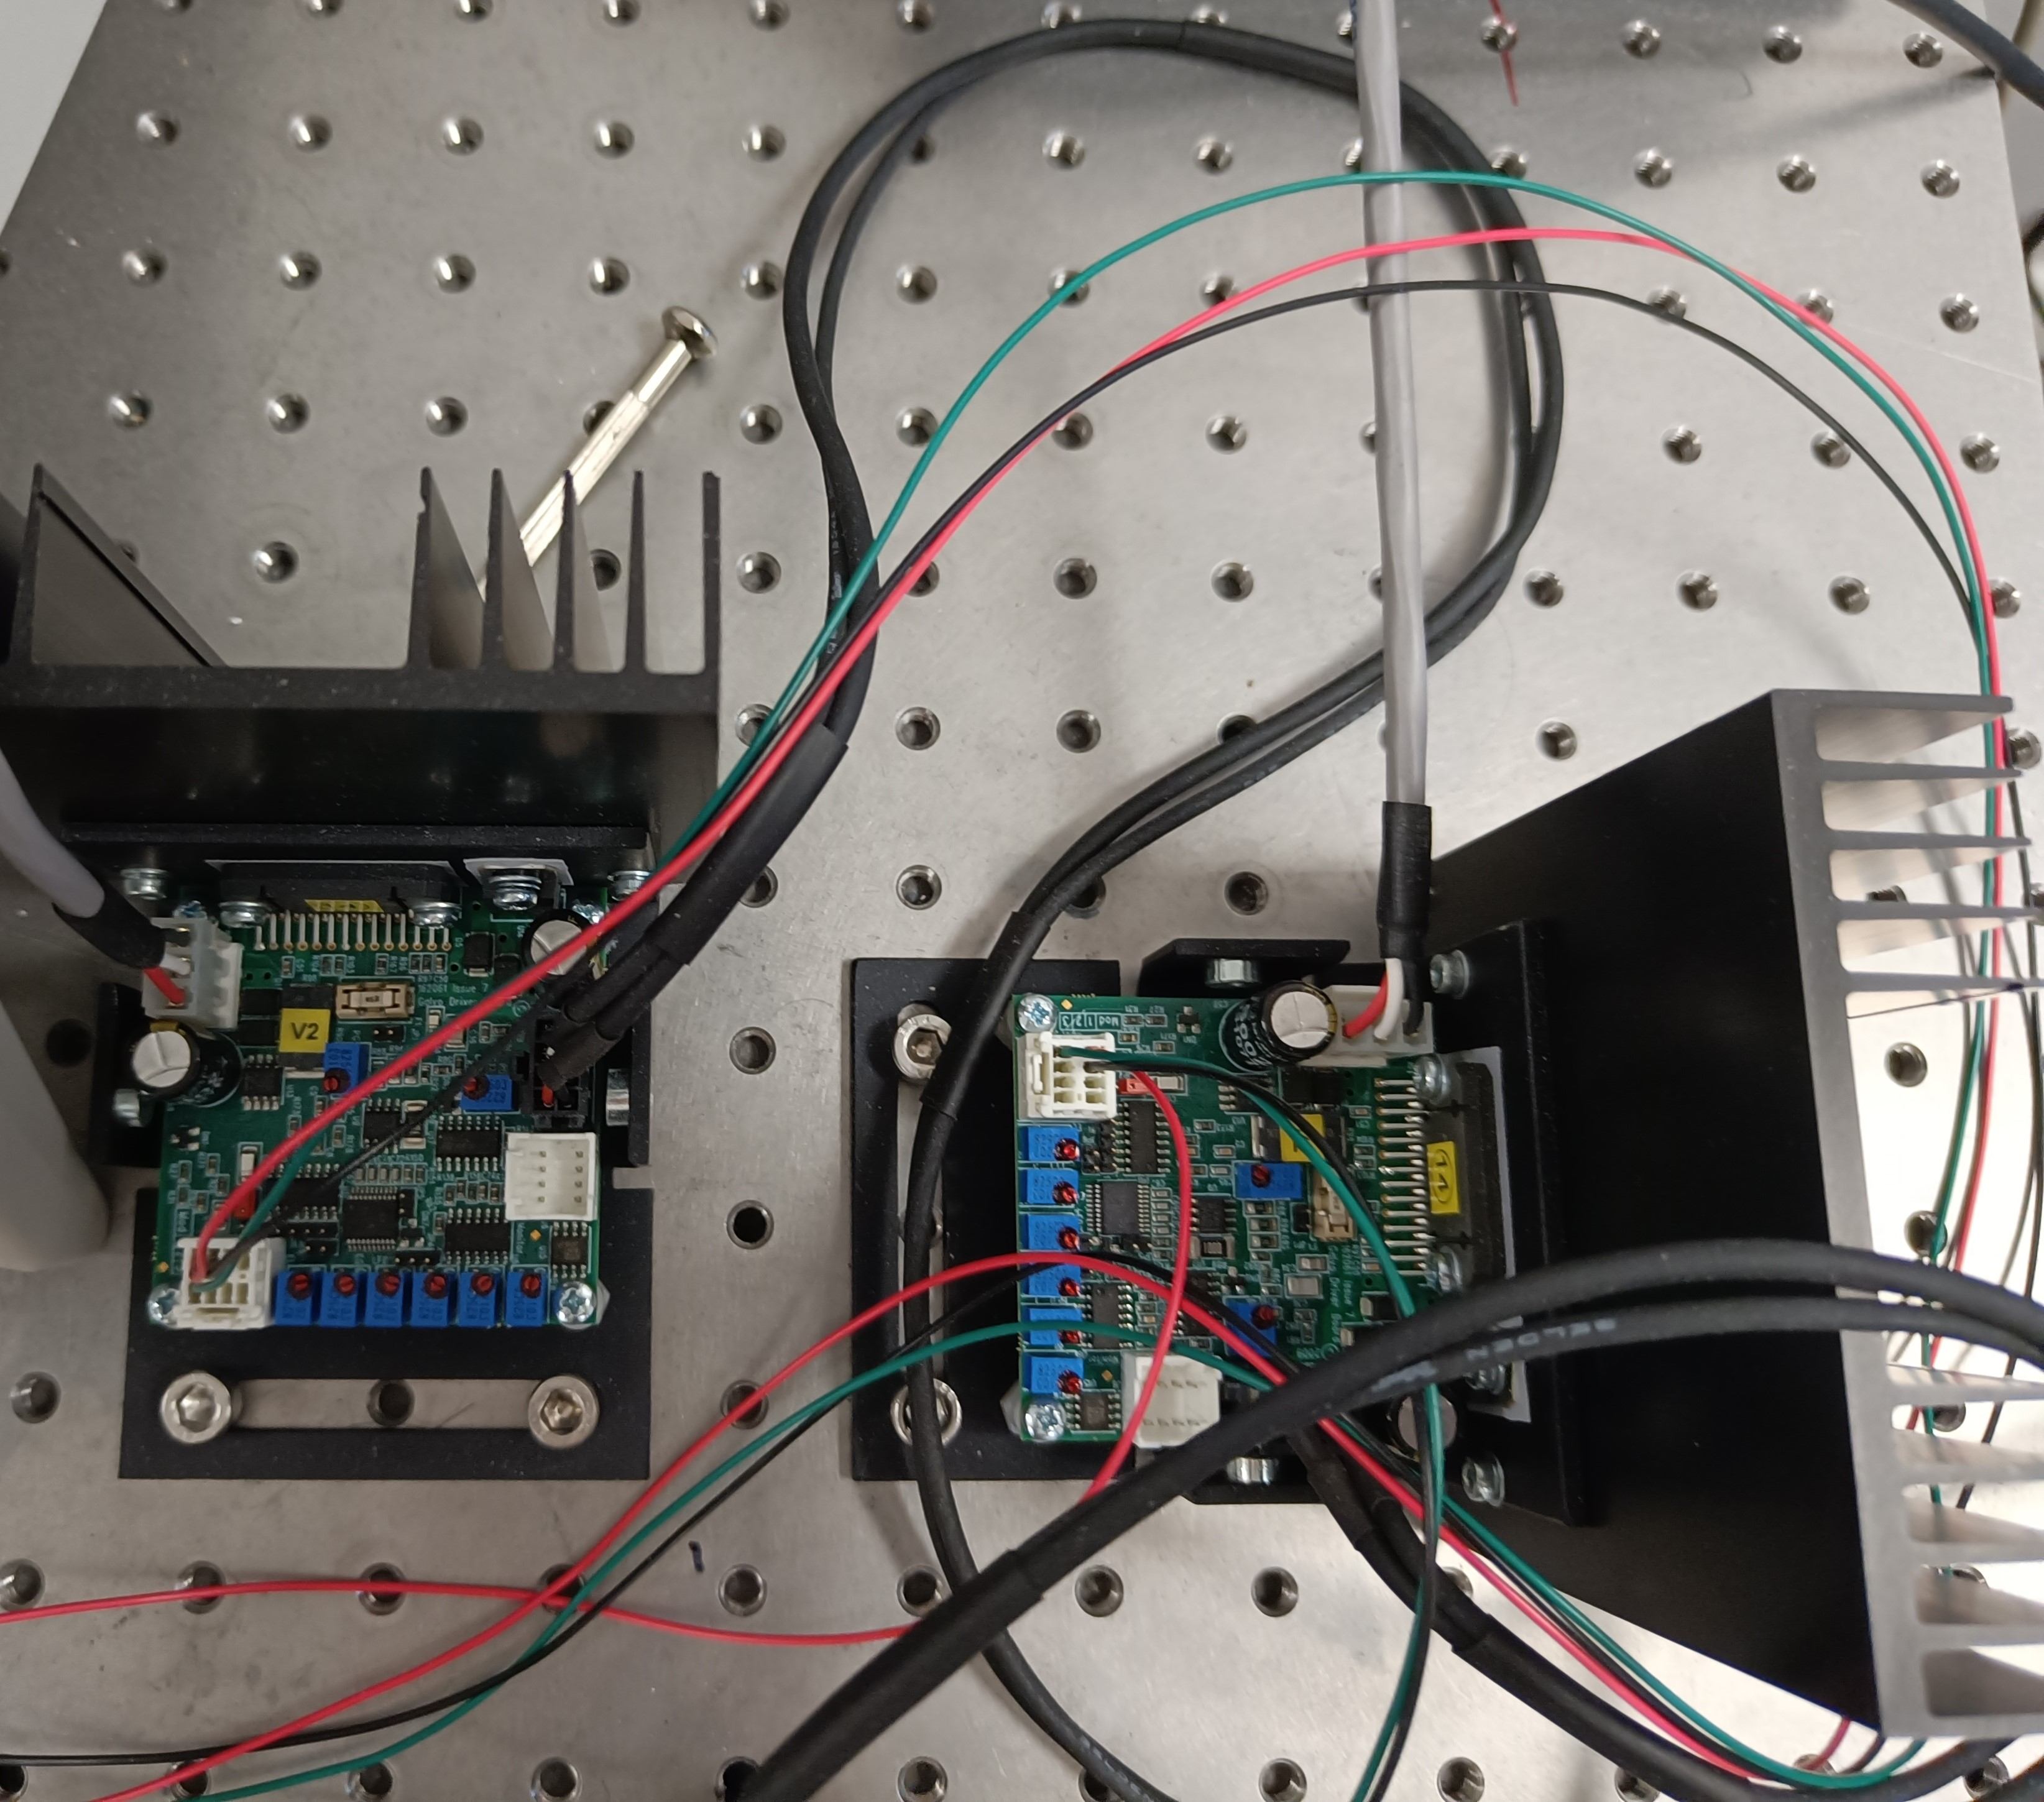
\includegraphics[width=\linewidth, height=0.7\linewidth]
		{galvano_mirror_controllers.jpg}
		\caption{}
	\end{subfigure}

	\caption{Signal generator galvano mirror controller, channel 1 controls the x-axis 
		mirror, while channel 2 controls the y-axis mirror. Both channels can be manipulated
		independently.}
	\label{fig:signal_generator}
\end{figure}

For our applications a 4f correlator is utilised to ensure that the 
motion of the galvano-mirrors does not move the focal point of the 
laser, allowing for a stable trap even while in motion. As shown in Fig.~\ref{fig:setup}, after the galvano-mirror we have our two lenses 
- $f_3$ and $f_4$ - the former being installed $150\ mm$ from the 
second mirror of the galvano, and the latter being installed $200\ mm$ 
from the back focal plane of the trapping objective. The signal 
generator used was supplied by 'MCS Test Equipment Ltd', allowing for 
dual channel signal control. This allowed us to precisely control the
alignment, amplitude, phase, and frequency of both mirrors making 
alignment much easier. 

While in theory the frequency can be increased until the mechanical 
limit of the mirrors is reached ($\approx 1000\ Hz$), the practical 
upper limit is determined by the trap strength. For a silica sphere 
this is on the order of $300\ Hz$ when suspended in water. Likewise 
while in theory the signal amplitude can be increased until the 
voltage limit of the motors is reached ($\approx 5.0 V$) the geometry 
of the focal lenses limits the maximum amplitude to $0.5 V$ as any 
greater will move the laser beyond the lens. For basic trapping 
calibration the galvano-mirrors were set to DC output, providing a 
fixed spot which operates like a typical optical trap.

%%%%%%%%%%%%%%%%%%%%%%%%%%%%%%%%%%%%%%%%%%%%%%%%%%%%%%%%%%%%%%%%%%%%%%%%%%%%%%%
%%%%%%%%%%%%%%%%%%%%%%%%%%%%%%%%%%%%%%%%%%%%%%%%%%%%%%%%%%%%%%%%%%%%%%%%%%%%%%%
\section{Synthesis of Birefringent Micro spheres}
\label{sec:vaterite}
There are several options for particles that can be rotated 
using optical tweezers \cite{Parkin2009, Saito2022}. Over 
the course of the project two different micro spheres where 
investigated, Vaterite and liquid crystal droplets. Both can 
be readily synthesised in the lab and are will rotate at a 
variety of sizes (see \ref{sec:opt_torque}).

Vaterite is a polymorph of calcium carbonate that is rarely 
seen in nature due to its low stability \cite{KonopackaLyskawa2019}. 
All three polymorphs are inherently birefringent meaning 
that they can be rotated using circularly polarised light. 
However unlike its other polymorphs of calcite and aragonite, 
when synthesised vaterite will typically form small spherical 
particles making them ideal for optical trapping and rotation. 
Synthesis of Vaterite micro spheres requires fine control of 
the crystal growth process in order to maintain polymorphic 
stability. Though for the purposes of optical rotation the 
exact polymorph is not as important as the morphology as all 
3 polymorphs are inherently birefringent. 

Vaterite samples where made by the first preparing equal amounts 
of $CaCl_2$ and $Na_2CO_3$ at a concentration of $0.33M$, at 
the same time a vial of $0.33M\ MgSO_4$ was prepared and set 
aside for later. First a small vial was filled with $1.5mL$ of 
$CaCl_2$ followed by $60\mu L$ and $90\mu L$ of $MgSO_4$ and 
$NaCO_3$ respectively, forming a seed solution. Next, a larger 
vial was filled with $5\ mL$, $1.5\ mL$, and $1\ mL$ of $CaCL_2$, 
$MgSO_4$, and $NaCO_3$ respectively followed by the seed solution. 
After 10 minutes of slow but continuous mixing a few drops of 
Agepon was added to halt the reaction, the solution was filtered 
and washed 3 times with distilled water before being suspended 
in water.
 
When trapped in circularly polarised light, the anisotropic 
crystal lattice allows spin angular momentum to be transferred 
to the Vaterite particle, resulting in a rotation about the 
beam axis. Because the particle scatters light anisotropically 
the signal detected by the QPD shows periodic fluctuations 
\cite{Yogesha2012}. In addition due to the change in polarisation 
there is also a periodic variation that appears at twice the 
rotational frequency \cite{Monteiro2018}. Therefore, the resulting 
power spectrum is not a Lorentzian but now also displays peaks 
that appear at integer multiples of the particles rotational 
frequency. 
\begin{figure}[h!]
	\centering
	\begin{subfigure}{0.4\linewidth}
		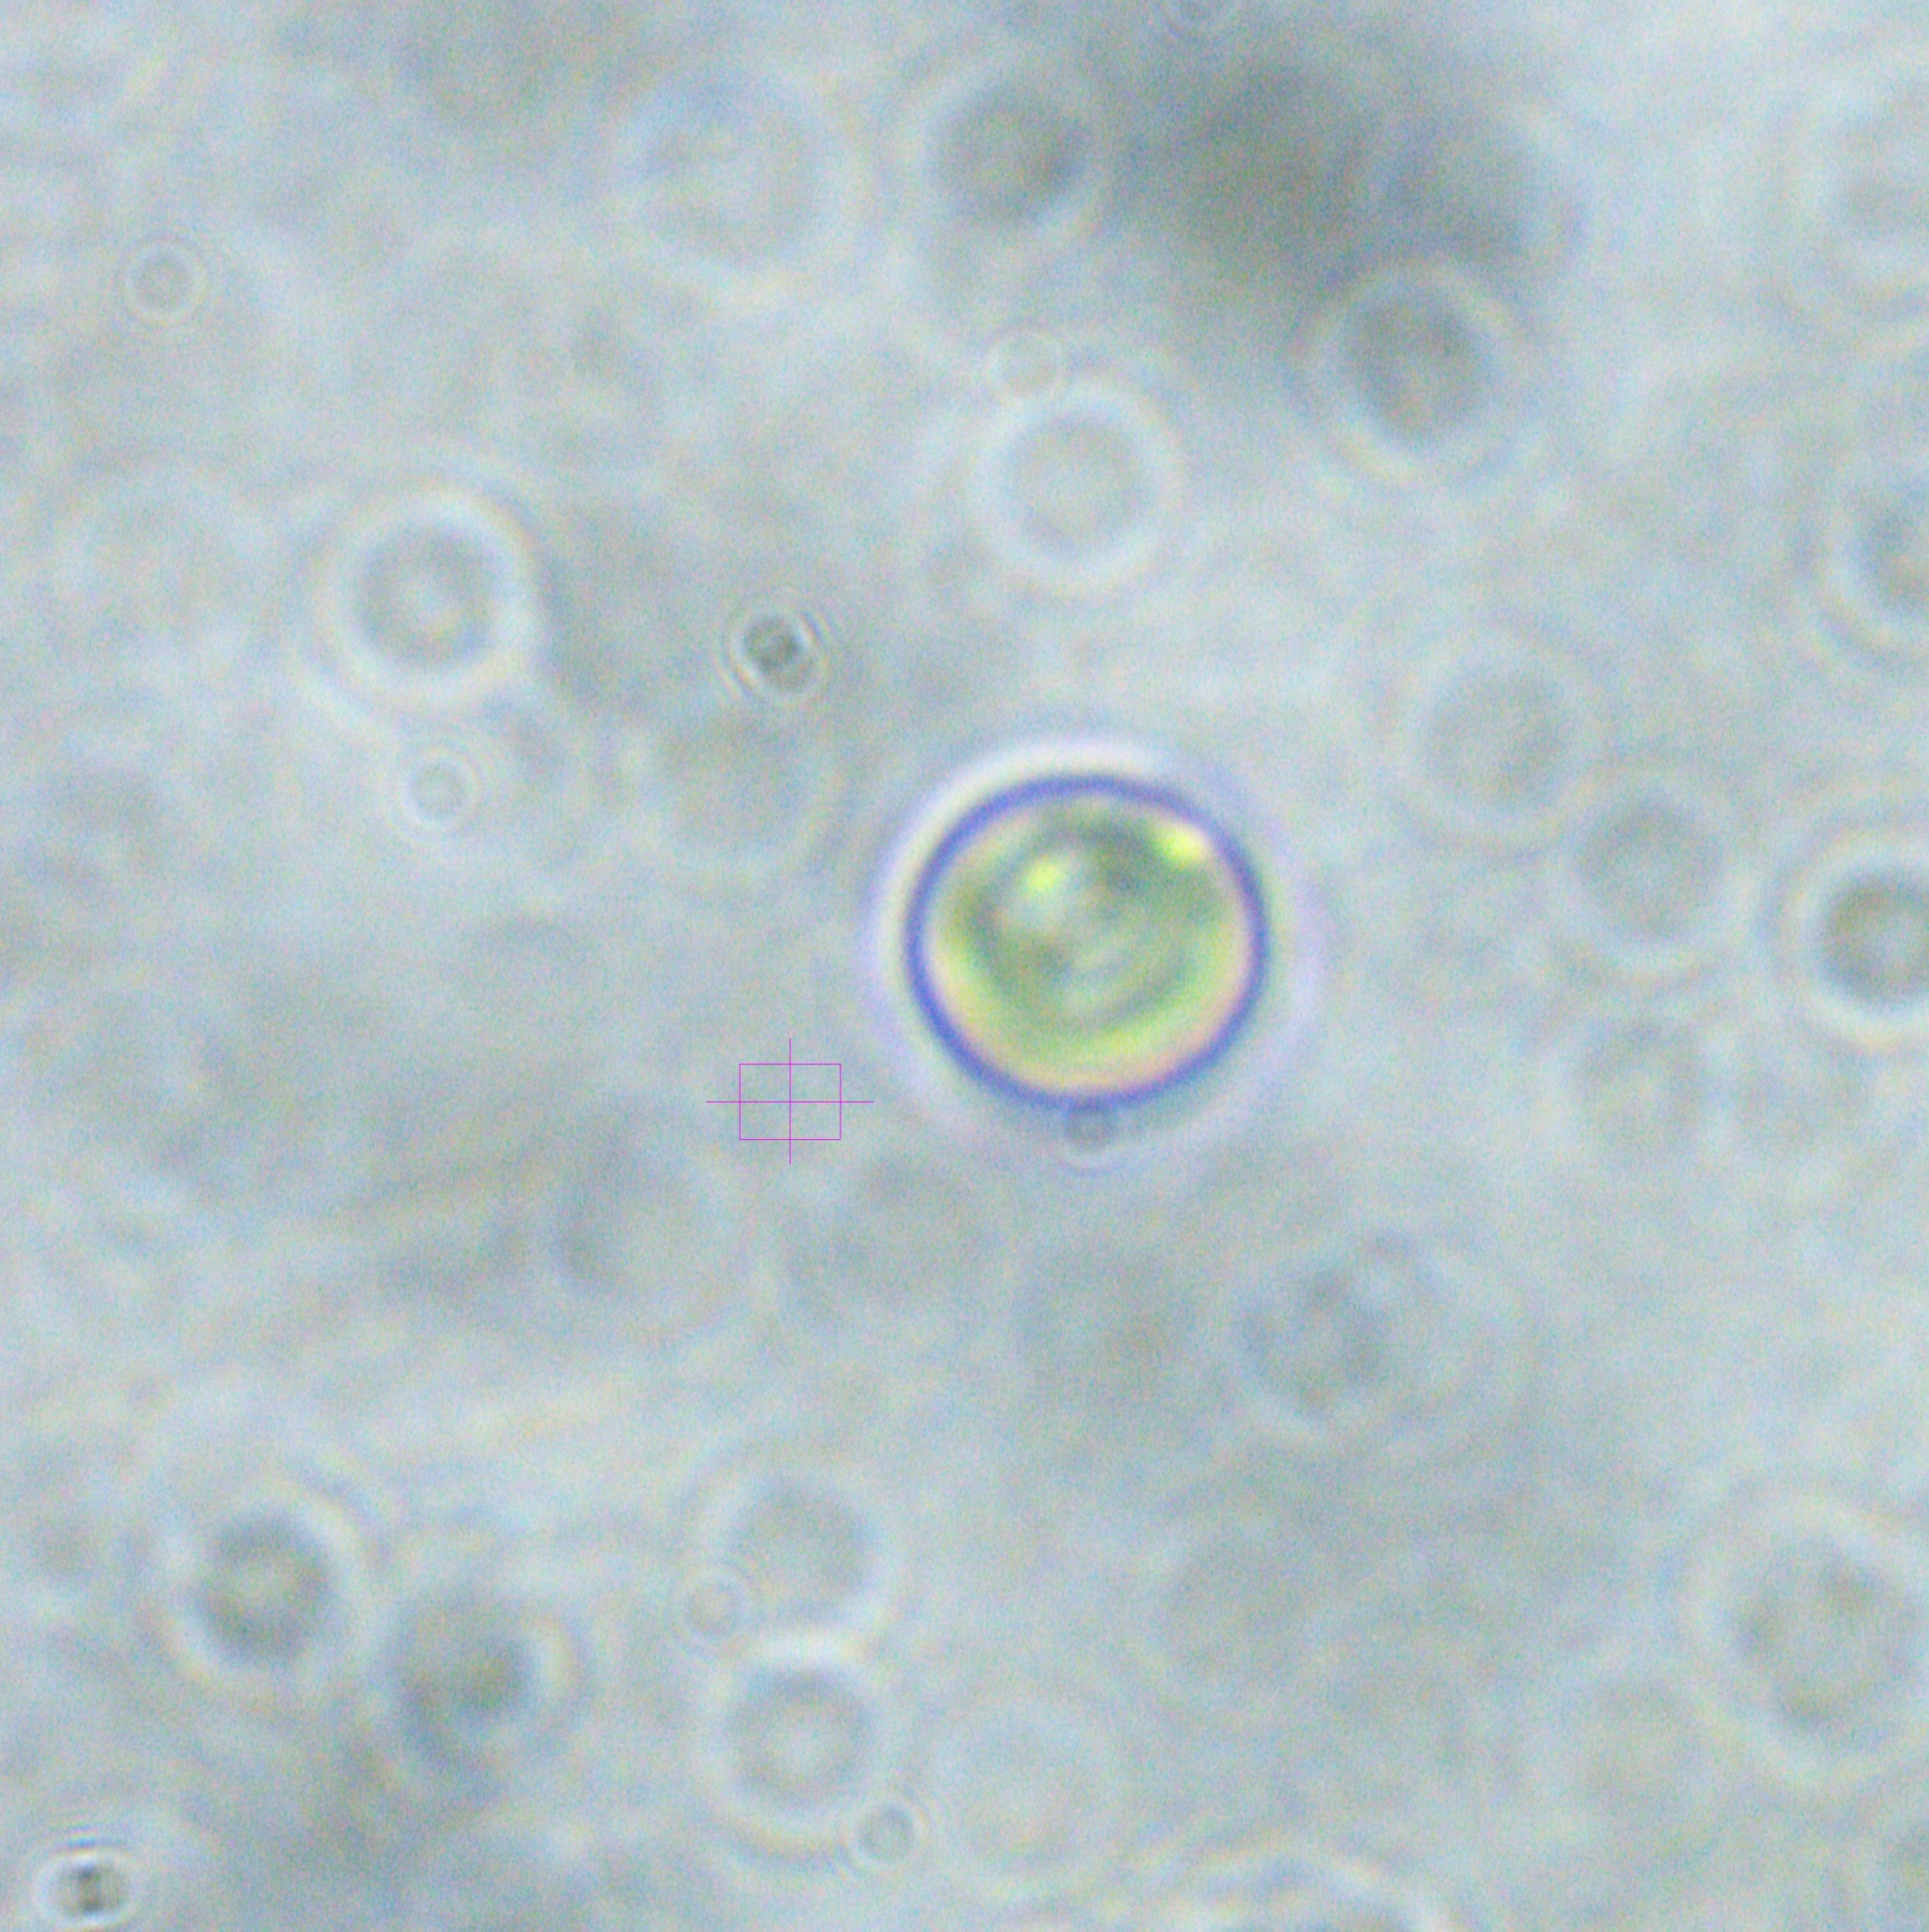
\includegraphics[width=\linewidth]{vaterite_sample.jpg}
		\subcaption{}
	\end{subfigure}
	\begin{subfigure}{0.55\linewidth}
		\includegraphics[width=\linewidth]{rotating_psd.png}
		\subcaption{}
	\end{subfigure}
	\caption{(a)Sample Vaterite sphere suspended in water and trapped by
		 circular polarised trap. (b) Collected power spectrum from 
		 rotating Vaterite, peaks in the power spectrum appear at integer 
		 multiples of the rotational frequency ($f_{rot} \approx 49.8$ Hz)}
	\label{fig:vaterite}
\end{figure}

As shown by Fig.~\ref{fig:vaterite}(b) the power spectra produced still 
demonstrates a Lorentzian curve but modified with these periodic peaks, 
while the Lorentzian can be loosely fitted to the end tail there exists 
no current model for describing the power spectra. The closest approximation
to this was conducted by \cite{Yogesha2012} where they describe the 
rotational motion of ellipsoidal polystyrene particles. The critical 
assumption being that the particle perfectly rotates in the $x-y$ plane. 
It has long been suspected that birefringent microspheres experience torques 
outside of the $x-y$ plane \cite{Volpe2023} making it very difficult to 
characterise the behaviour of rotating birefringent microspheres without a 
proper understanding of the full optical torque being applied to it.

\subsection{Liquid Crystal Rotors}
Liquid crystals are an intriguing example of materials with mixed phase
properties. Unlike typical solutes such as Glycine, a liquid crystal
can still maintain some degree of order between its individual molecules
while in the liquid state. This is due to the fact that liquid crystals
are constructed of ordered molecules that demonstrate a long range
ordering. There are three main types of liquid crystal transition methods:
Thermotropic crystals will transition to their liquid crystal phase when 
sufficiently heated. Lyotropic materials can undergo this transition due 
to changes in temperature and concentration. And lastly, Metallotropic 
materials - which are composed of both organic and inorganic molecules - 
change phase according to the ratio of organic to inorganic molecules present.
Liquid crystal rotors are rather simple in their production, 
4-Heptyl-4-biphenylcarbonitrile (7CB) was purchased from Sigma Aldrich
and a small amount was added to a vial of distilled water. The solution 
was then heated in a water bath to $25^\circ$ in order to transition the
solid crystal into its liquid crystal state. The solution can then be 
loaded onto a sample cover slip and the individual droplets visualised.
The molecules of 7CB will align with a strong electric field, and due to
the spherical droplet geometry the droplets are inherently birefringent. 
\begin{figure}[h!]
	\centering
	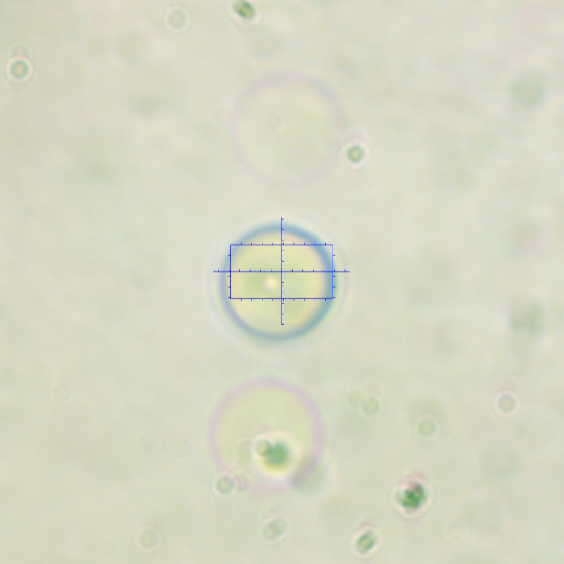
\includegraphics[width=0.5\linewidth]{LC_sample.png}
	\caption{Liquid crystal undergoing rotation due to the circularly polarised trap.} 
\end{figure}

The liquid crystal droplets had a much faster rotation rate than comparable 
Vaterite spheres, due to their higher degree of birefringence and the fact
that the droplets are far closer to perfect spheres making angular momentum
transfer more efficient. 

%%%%%%%%%%%%%%%%%%%%%%%%%%%%%%%%%%%%%%%%%%%%%%%%%%%%%%%%%%%%%%%%%%%%%%%%%%%%%%%
\section{Rotation of birefringent micro spheres} 
Optical tweezing has often been used for micro-rheology, by computing the
exact forces being exerted on the trapped sphere, one can determine the
local temperature/viscosity of the medium \cite{Millen2014, RodriguezSevilla2018}.

When it comes to optical rotation, a rotating particle will experience a
fluid drag torque that is proportional to its rotation rate, the maximum 
rotation rate is when the fluid drag is equal to the optical torque 
of the laser \cite{RodriguezSevilla2018}. Optical rotors have been used
to measure local temperature changes \cite{Millen2014}, or for understanding 
how fluid shear propagates through a medium \cite{Knoener2005}. Likewise, 
one can use a beam steering arrangement to probe the drag force of the 
fluid, by understanding the trap strength (calibrating using a low 
frequency signal) one can measure the drag force experienced by the local 
fluid \cite{RobertsonAnderson2018}. I

For any discussion of fluid flow its important that we know the fluid 
regime which is given by the Reynolds number. For a sphere submersed in a 
moving fluid of velocity $U$ this is given by:
\begin{align}
	Re = \frac{\rho UD}{\mu}
\end{align}

Where $D$ is the sphere's diameter, and $\rho$ and $\mu$ are the fluid's 
density and viscosity respectively. In our case we do not have a fluid
moving around a sphere but a sphere moving through the fluid at some 
velocity $U$, assuming a no-slip boundary condition we can model the 
fluid velocity profile based on the velocity of the particle. Assuming
that for now the fluid properties are unaffected by the rotating particle
we see that for an individual sphere the Reynolds number can only change 
due to increasing/decreasing the fluid velocity. The fluid velocity is 
directly proportional to the particles rotation rate for low Reynolds
numbers \cite{Bruce2020}. Given the small size of the particles used 
($1-10\mu\ m$ in diameter), and the relatively low rotation rates that 
are possible with an optical tweezer, for the case of our analysis the
Reynolds number will not never be large enough to consider factors such
as turbulence. There are two possible avenues for generating shear flow 
with a trapped particle; rotation of birefringent particles, and fluid 
flow induced by particle motion. 

Rotating birefringent particles are the more common method for generating 
and measuring fluid flow in a solution. To see if we can even achieve the 
theoretical maximum shear rate, Vaterite spheres were synthesised (see 
Sec.\ref{sec:vaterite}) submerged in water and trapped with the 1064 nm 
laser at set to 450 mW. The rotation frequency was determined using the 
QPD, and the particle sizes were computed by image analysis. With the 
particle size and rotation frequency, the tangential rotation speed is 
calculated via:
\begin{align}
	\label{eq:birefringent_speed}
	u(r) = \frac{\pi}{4}\frac{d^3}{r^2}\omega
\end{align}

Where $d$ is the particle diameter, $\omega$ is the rotation frequency
reported by the QPD, and $r$ is the distance from the particle's centre. 
Using Eq.\ref{eq:birefringent_speed} we calculated the fluid flow radiating
outward from the centre of the sphere. The shear rate can then be computed
as the partial derivative fluid flow (assuming shearing is generated purely
by the flow field). This approach was used previously with liquid crystal 
rotors \cite{Saito2022}:
\begin{align}
	\label{eq:birefringent_shear}
	\dot{\gamma}(r)=\left|\frac{\delta u(r)}{\delta r} \right|= 
	\frac{\pi}{2}\frac{d^3}{r^3}\omega
\end{align}

One would expect that we set some reference distance where the fluid flow 
would be considered zero. However, at a microscopic level we are more 
concerned by the fluid shear for an individual nucleation event. We are
essentially computing what the shear rate would be for a small volume 
of fluid between two moving parallel plates. This is similar logic to Mura 
and Zaccone's work where they considered the shear on a subcritical nucleus
in a flow field \cite{Mura2016}. They go further in depth to discuss the 
impact of material transport, overall coming to the conclusion that 
increasing shear rate leads to an increase the nucleation rate up till some
maximum. 
%%%%%%%%%%%%%%%%%%%%%%%%%%%%%%%%%%%%%%%%%%%%%%%%%%%%%%%%%%%%%%%%%%%%%%%%%%%%%%%%
%%%%%%%%%%%%%%%%%%%%%%%%%%%%%%%%%%%%%%%%%%%%%%%%%%%%%%%%%%%%%%%%%%%%%%%%%%%%%%%%
\subsection{Estimation of fluid flow around a rotating particle in bulk fluid}
First we determined the upper rotation rate that could be achieved 
using both Vaterite and liquid crystal spheres. Vaterite samples 
were synthesised according to \cite{Parkin2009, Bishop2004} (see 
sec.~\ref{sec:vaterite}), and then suspended in distilled water. 
A sample of $200\ \mu L$ was pipetted and a single microsphere was 
captured via a circular polarised beam. 

Due to Van der Waal's forces some of the microspheres were stuck 
together, fortunately individual sphere's were still present. 
Individual microspheres were trapped and their rotation rate was 
determined by looking at the peak frequency component of the 
collected power spectrum. Due to their anisotropic scattering the 
QPD signal will oscillate periodically. After taking the Fourier
transform of the QPD signal the power spectrum has distinctive
peaks at integer multiples of the rotational frequency. The largest 
peak is often twice the rotational frequency which is due to the 
polarization modulation of the scattered field, the first peak 
is due purely to the rotation of vaterite sphere \cite{Monteiro2018}. 
An example of this is behaviour is shown in fig.~\ref{fig:tdat_fdat}.

\begin{figure}[h!]
	\begin{subfigure}{0.49\linewidth}
		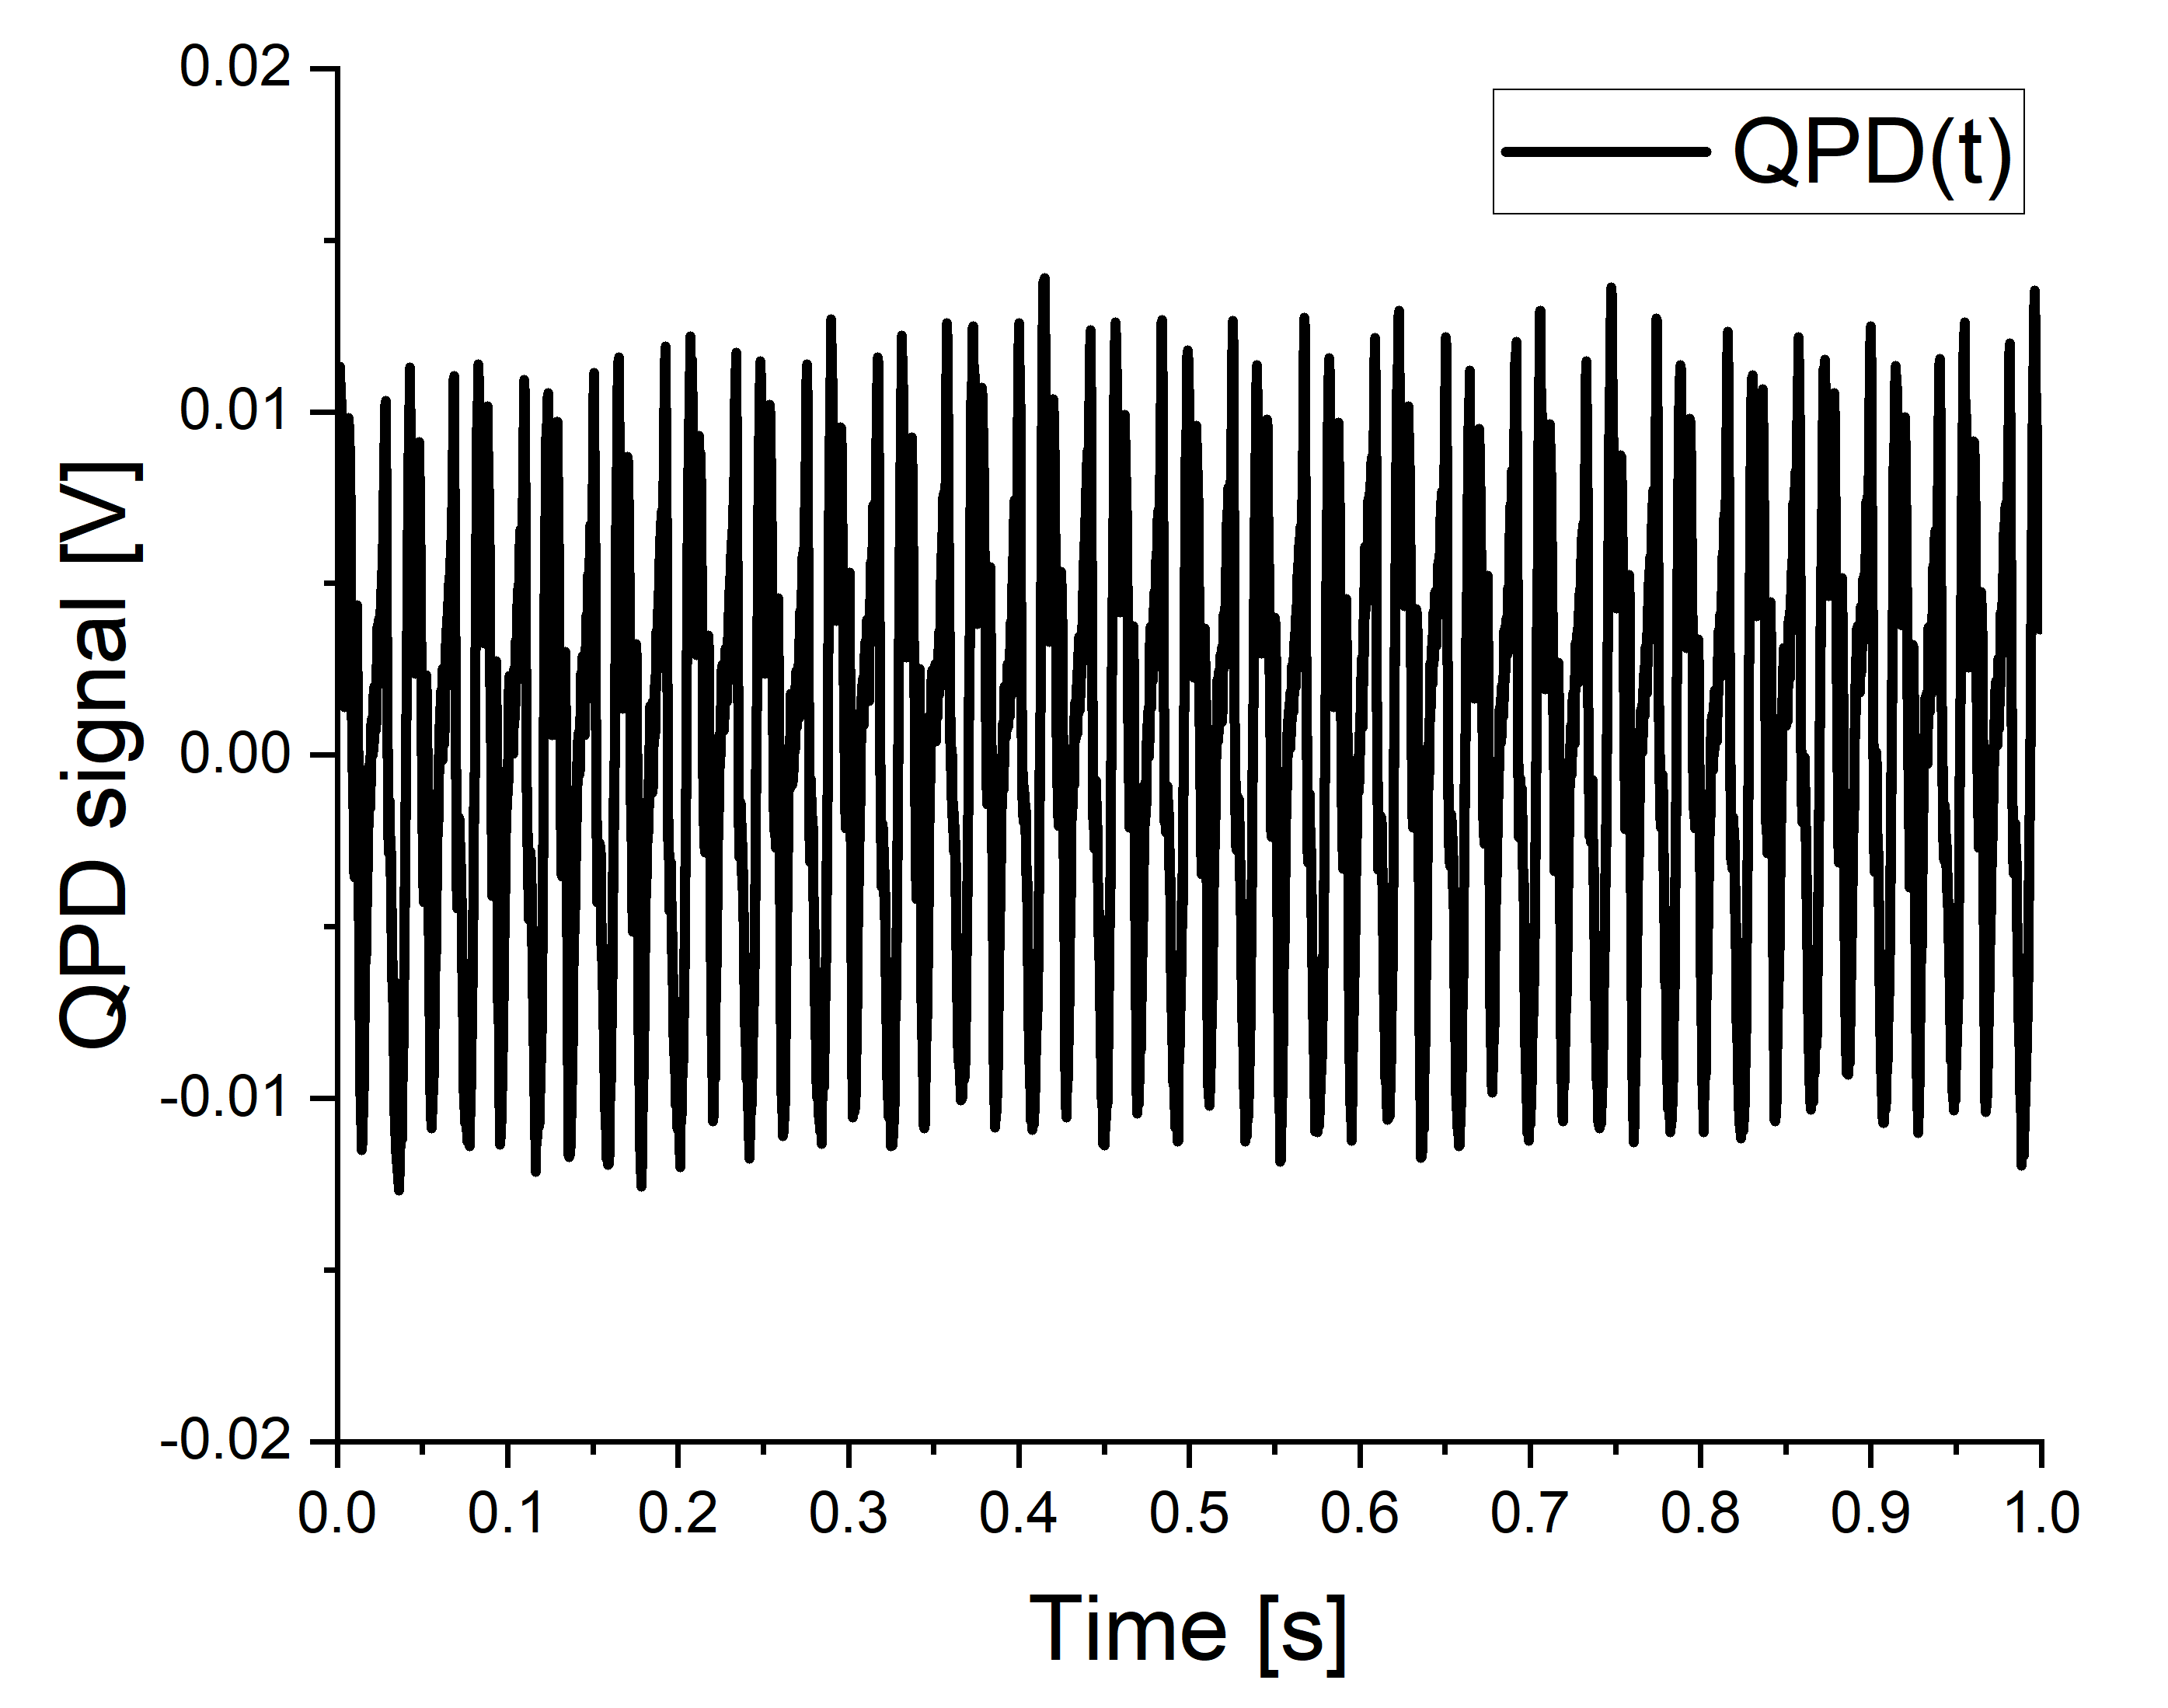
\includegraphics[width=\linewidth]{time_domain_data.png}
	\end{subfigure}
	\begin{subfigure}{0.49\linewidth}
		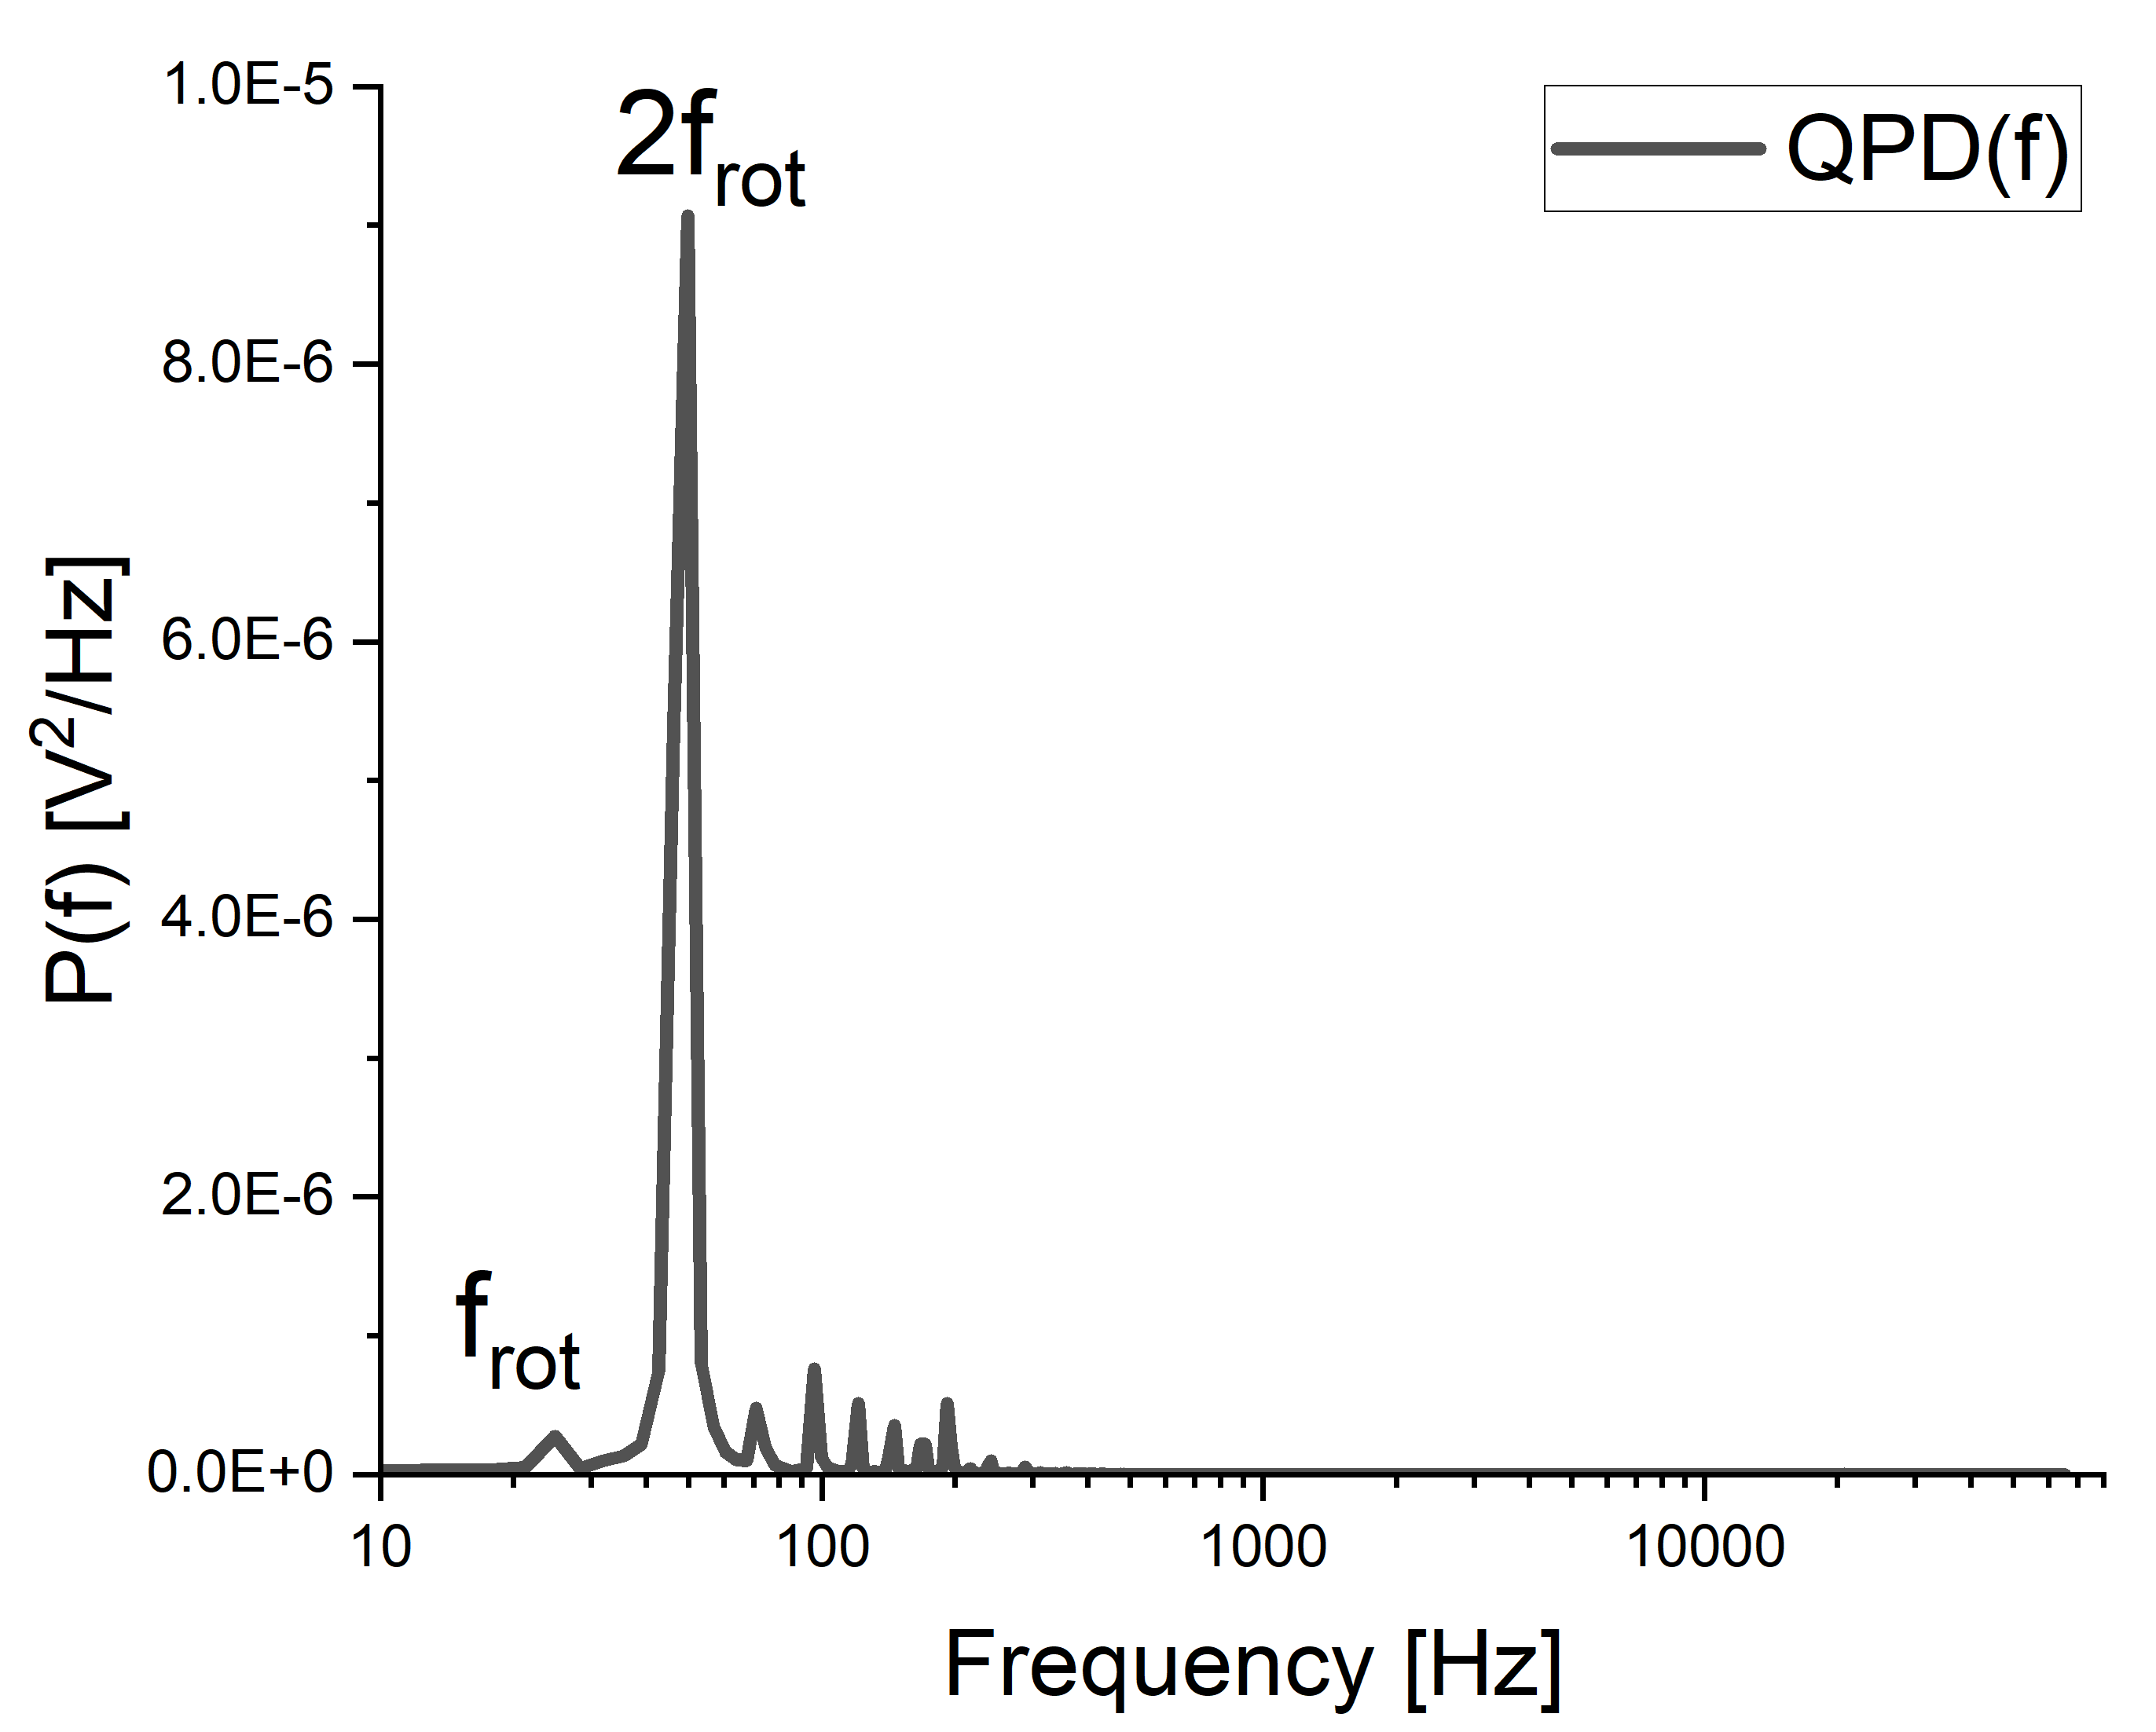
\includegraphics[width=\linewidth]{frequency_domain_data.png}
	\end{subfigure}
	\caption{Example of QPD signal being converted from the time 
		domain to the frequency domain. (left) Raw signal collected
		from the QPD over the 1st second of its trajectory showing 
		a periodic spacing with a period of $1/f_{rot}$. (right) 
		Power spectrum of the QPD signal, the y-axis is a linear 
		scale to demonstrate the clear peaks in the power spectra. 
		The rotational frequency is the first instance of a peak 
		forming, and after that the peaks appear in integer 
		multiples of $f_{rot}$}
	\label{fig:tdat_fdat}
\end{figure}

The accuracy of the rotational frequency is dependent on the sample
rate of the QPD and the sample duration \cite{BergSoerensen2004}. 
With higher sampling rates resulting in a wider frequency window 
(see Sec.\ref{sec:psd}) and longer sampling durations resulting in 
more distinct rotational peaks. The default QPD sampling rate is 
$2^{17}\ Hz$ which is more than adequate for detecting even the 
slightest low frequency signals. And the default sampling duration 
was $3\ s$ which for most cases gave us clear distinct peaks for 
even relatively low rotational frequencies. After trapping a 
vaterite microsphere the power spectrum was recorded and the 
rotation frequency was acquired. This was repeated several times
for each sphere trapped, to confirm that the rotational frequency
was constant and that the sphere had reached its maximum rotation 
rate.
    
After computing the rotational frequency the radial fluid speed 
could be estimated using Eq.~\eqref{eq:birefringent_speed}. From 
there we can estimate the shear flow experienced by a small volume 
of fluid within the flow field (see Eq.\eqref{eq:birefringent_shear}). 
Here we only consider the fluid flow as it propagates outward from 
the axis of rotation. While the cover slip will have some effect 
fluid flow it is difficult to quantify the effects of a hard 
boundary on a rotating object when the boundary is perpendicular to 
the axis of rotation. 
\begin{figure}[h!]
	\centering
	\begin{subfigure}{0.7\linewidth}
		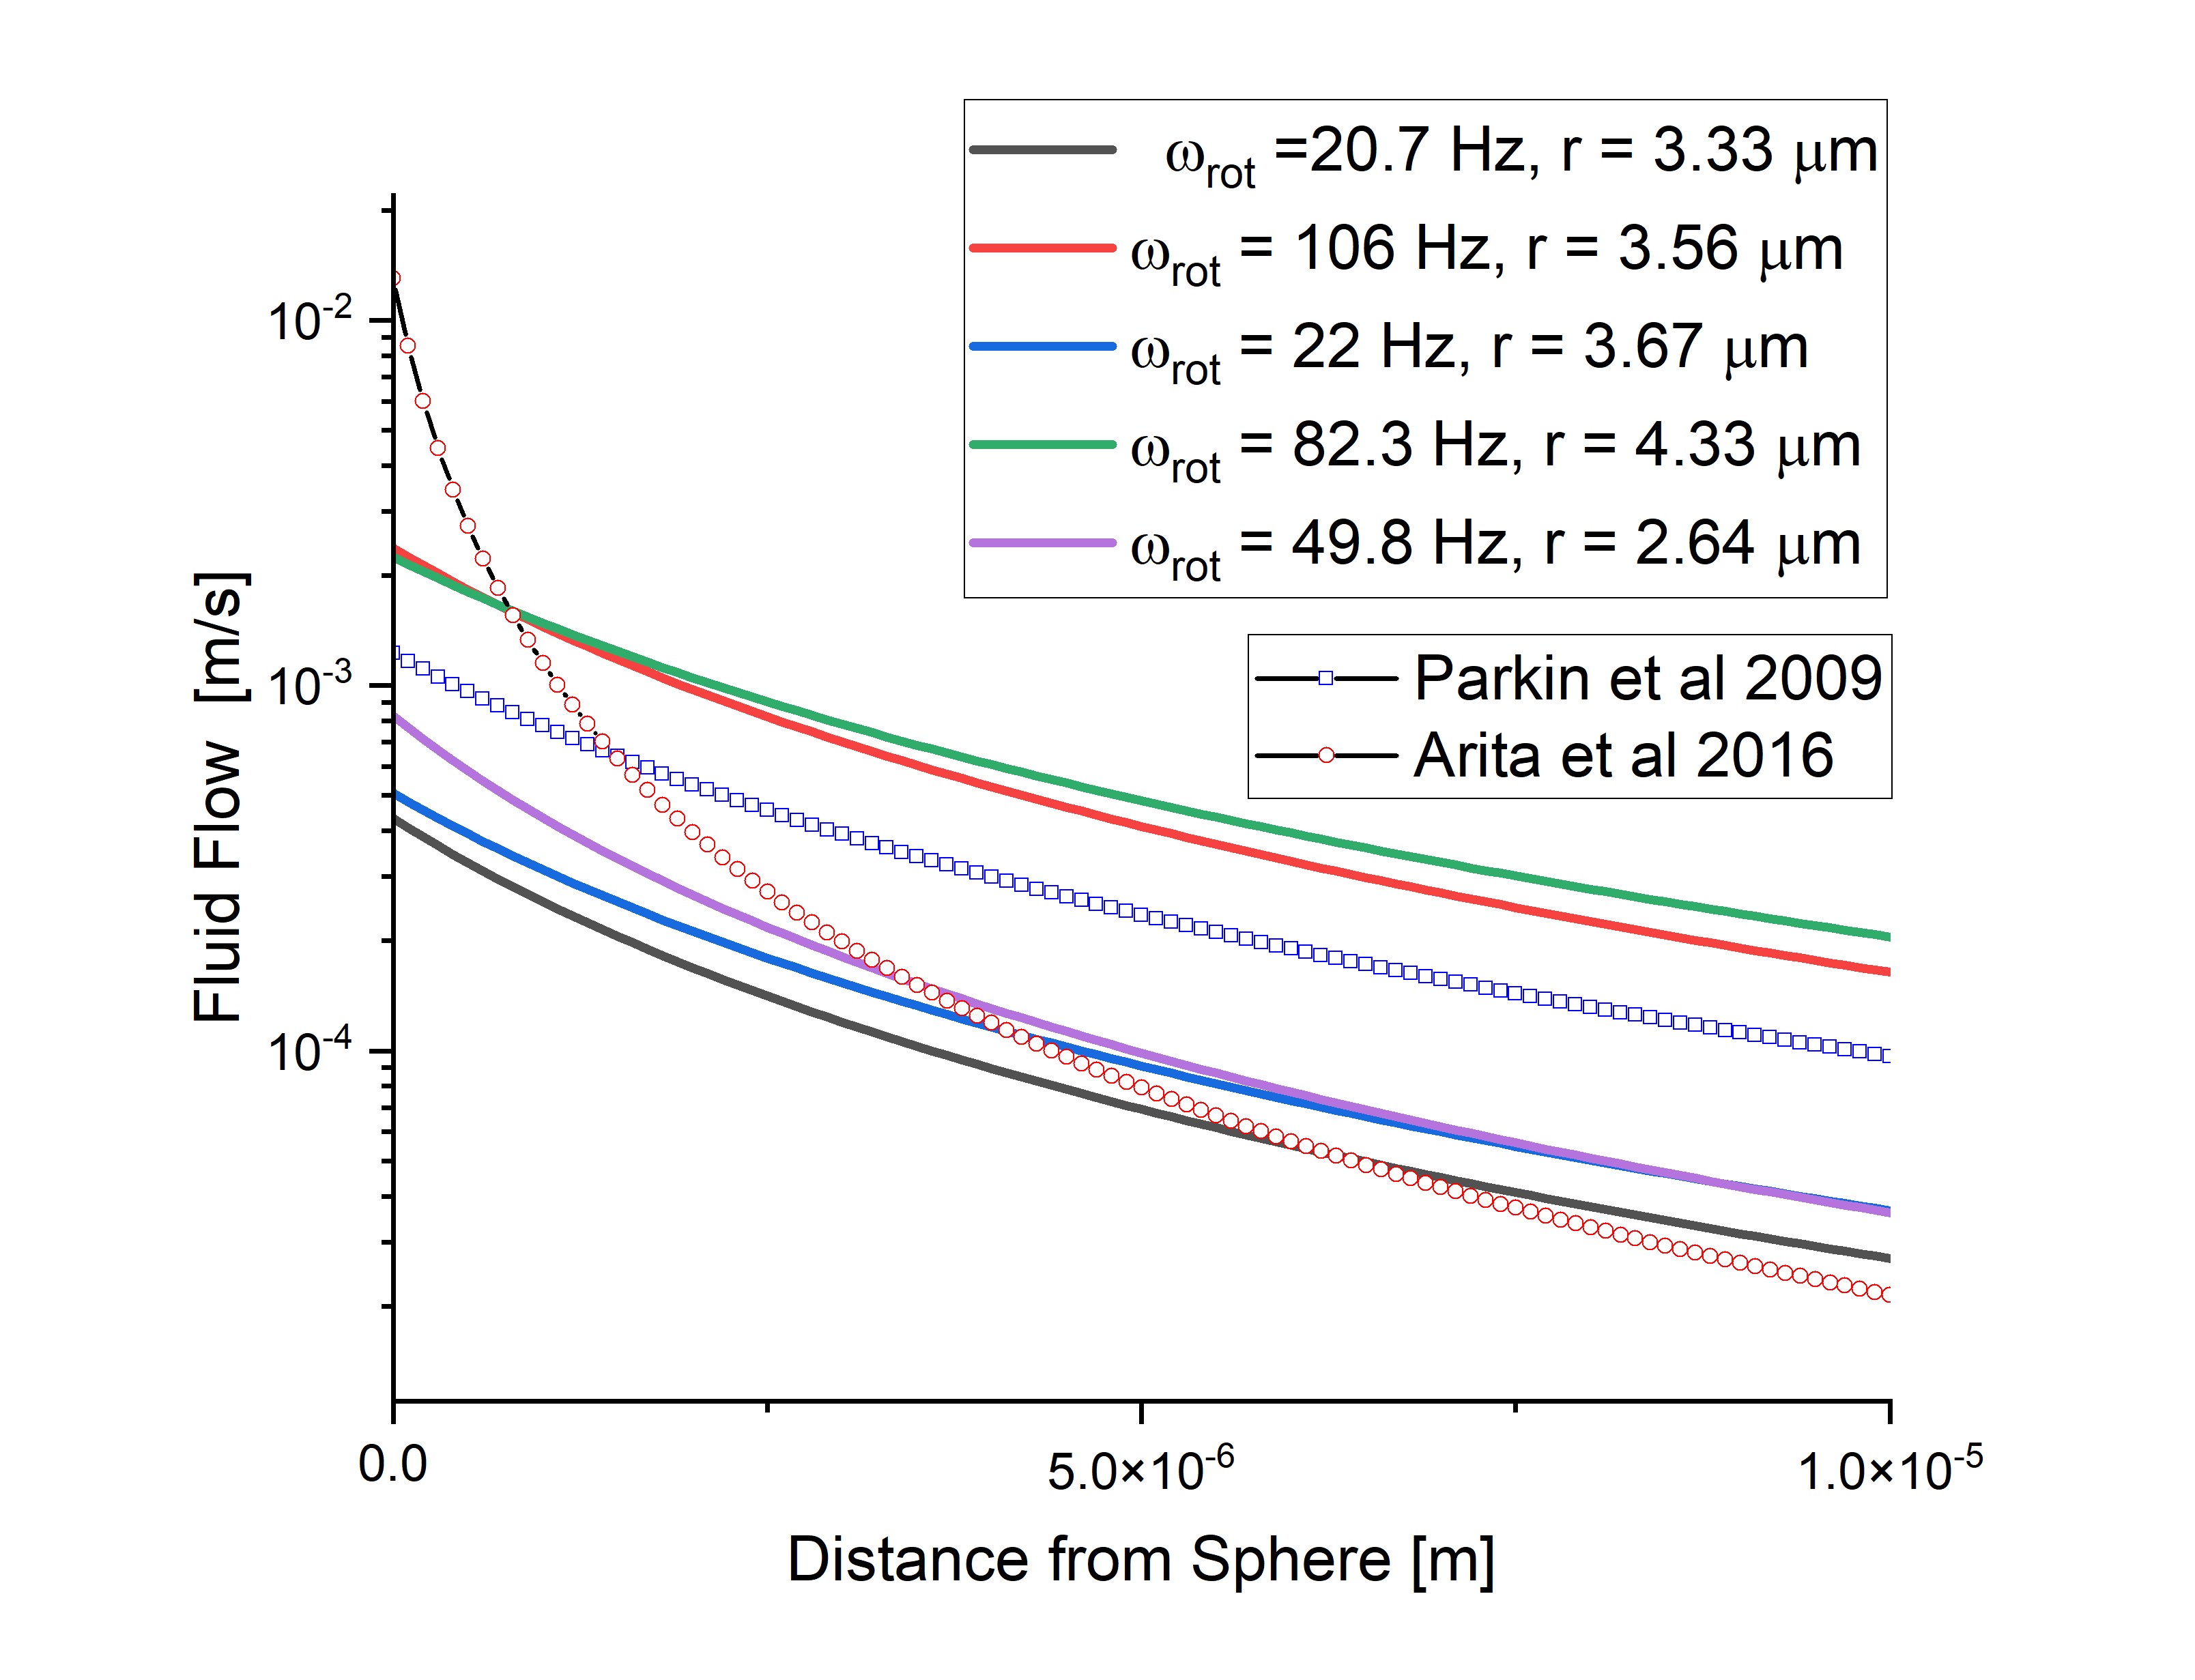
\includegraphics[width=\linewidth]{vaterite_fluid_flow.png}
		\caption{}
	\end{subfigure}
	\begin{subfigure}{0.7\linewidth}
		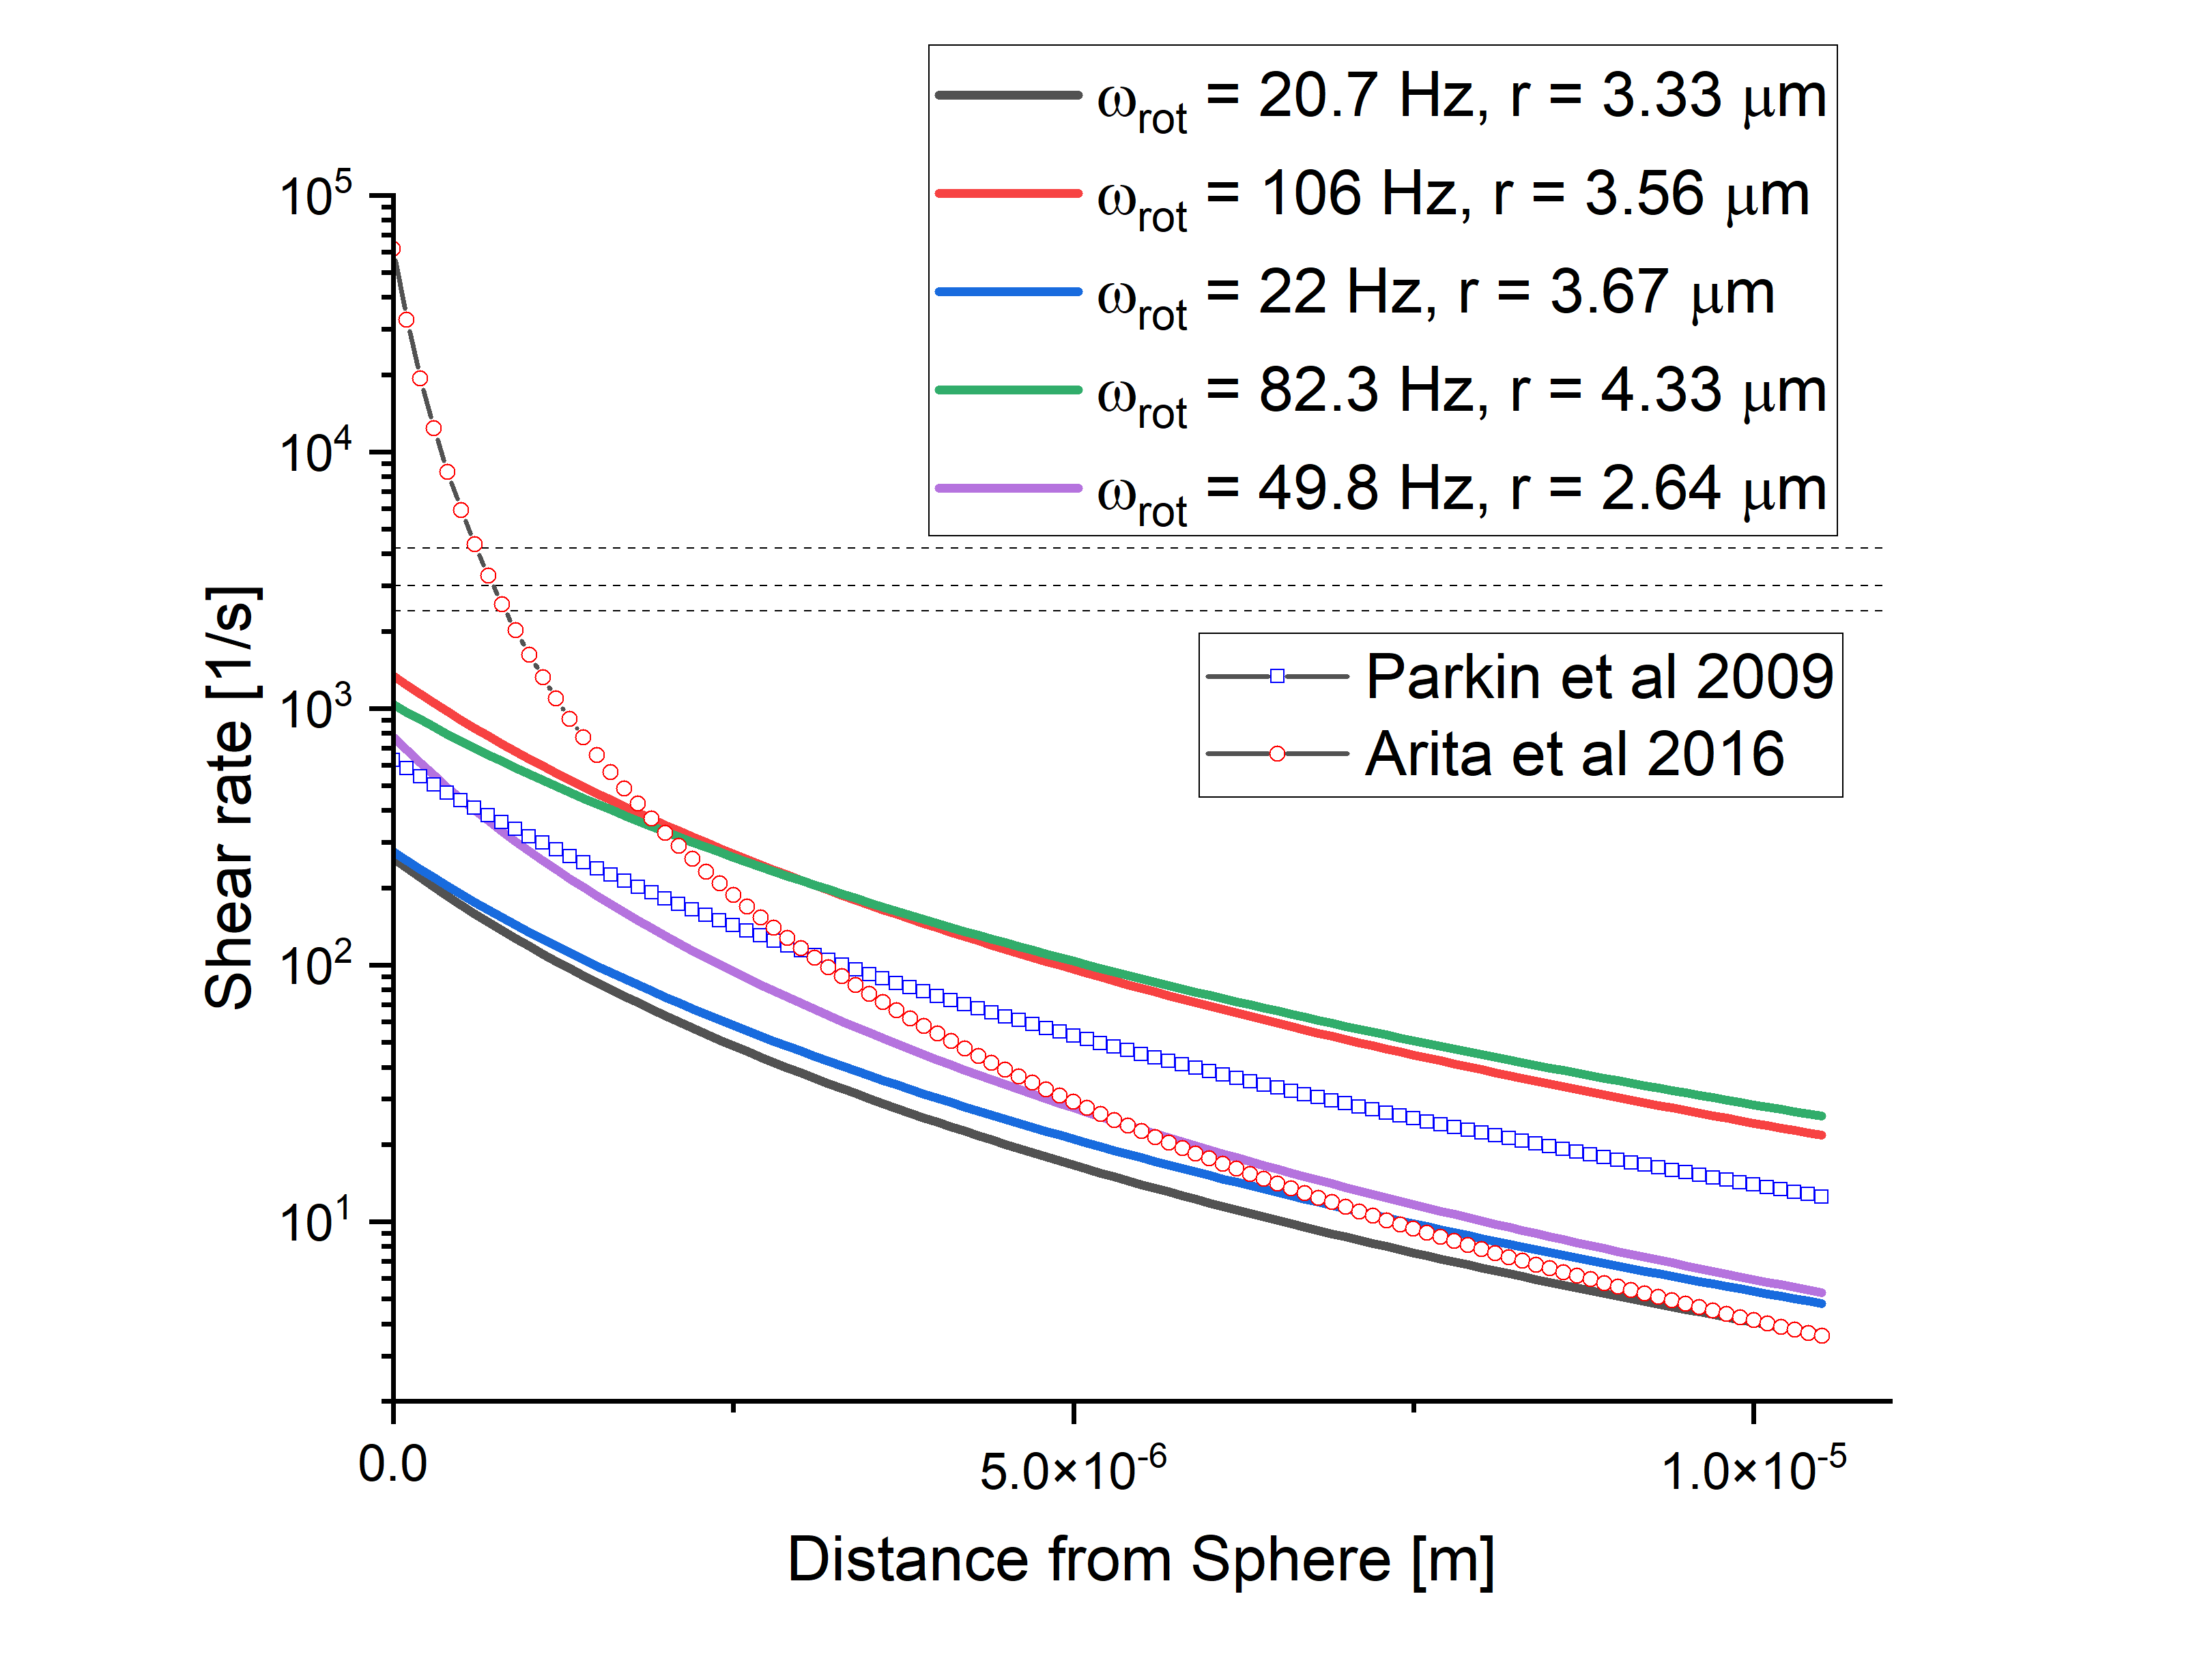
\includegraphics[width=\linewidth]{vaterite_shear_rate.png}
		\caption{}
	\end{subfigure}
	\caption{(Top) Fluid flow radiating out from the surface of a
		rotating Vaterite sphere. (Bottom) Shear rates computed 
		using Eq.\ref{eq:birefringent_shear}, optimal shear rate is 
		of $3000 s^{-1}$ is indicated by the dotted line. Vaterite 
		radii and rotation frequencies are shown, the laser power 
		was kept constant at 450 mW. Reported rotation rates, and 
		their corresponding fluid flow and shear rates, for Vaterite 
		are also plotted alongside lab results. Results from 
		\cite{Parkin2009, Arita2016} are included as well.}
	\label{fig:vaterite_shear}
\end{figure}

From Fig.\ref{fig:vaterite_shear} there is not a strong relationship 
between particle size and rotation rate, this is contrary to much of 
the theoretical predictions that predict an exponential decay with 
particle size. This can be in part due to the fact that synthesising 
perfectly spherical spheres that have uniform birefringence across the 
whole population is difficult. Despite our best efforts at controlling 
the growth rate the smallest particle ever synthesised was around $3\ 
\mu m$ in diameter. The Vaterite spheres would often stick together 
while suspended in water after a short period of time. The fastest 
reported rotation rate within a fluid was by \cite{Arita2016} 
that achieved a rotation rate of $5\ kHz$, this is plotted in Fig~\ref{fig:vaterite_shear}. In addition we added the results from 
\cite{Parkin2009} as a more realistic example. 

The optimal shear rate predicted by \cite{Debuysschere2023} is 
plotted on Fig.~\ref{fig:vaterite_shear}(b), the outer dotted 
lines represent the point when the nucleation rate is less than 
90\% of the maximum. We can visualise the fluid around the 
rotating sphere by dividing it up into radial sections. Assuming 
the sphere is rotating sufficiently quickly there are three 
sections of concern, as demonstrated by fig.~\ref{fig:shear_diagram}. 
The fluid close to the sphere experiences a shear rate that 
is far greater than the optimal shear rate, in which case 
nucleation is suppressed \cite{Mura2016}. Secondly, there is 
a region of fluid that experiences a shear rate close to the 
optimal value ($\pm 5\%$) where the nucleation rate is enhanced 
significantly compared to the bulk fluid. Lastly, beyond the 
optimal region the shear rate drops off exponentially in which 
case the nucleation rate is barely different compared to the 
bulk fluid.
\begin{figure}[h!]
	\centering
	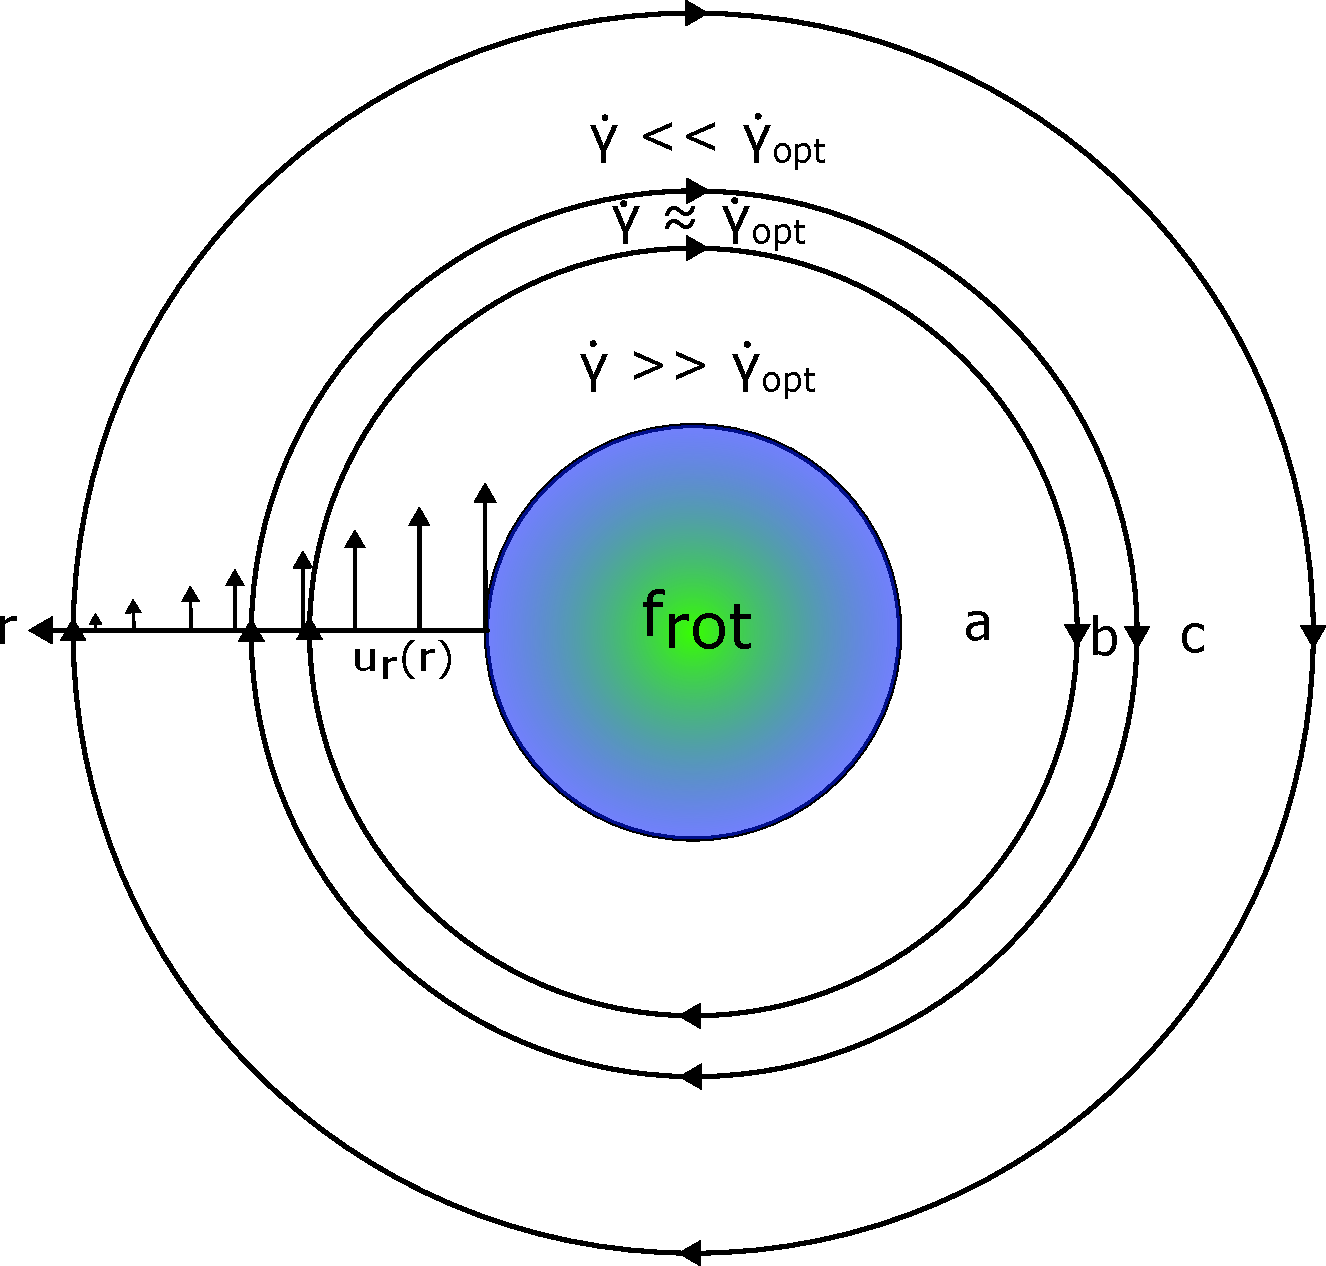
\includegraphics[width=0.875\linewidth]{shear_rate_diagram.pdf}
	\caption{Diagram demonstrating how fluid shear rate varies 
	radially from a rotating sphere (rotation rate = $f_{rot}$). 
	(a) the shear rate exceeds the optimal shear rate 
	($\dot{\gamma}_{opt}$) and suppresses the nucleation rate. 
	(b) shear rate is close to the optimal amount, enhancing the 
	nucleation rate. (c) shear rate is far below the optimal 
	amount and the nucleation rate is comparable to the bulk fluid.}
	\label{fig:shear_diagram}
\end{figure}

\section{Rotating spheres in Supersaturated solution}
If rotation rates in bulk solution are insufficient then a 
rotating sphere close to an artificial barrier may be able 
to improve the shear rate of the surrounding fluid. Of course 
placing a solid barrier in a supersaturated fluid may well 
encourage nucleation somewhere on the surface outside of our 
control. Instead we chose to use the droplet edge of the 
supersaturated solution, while not a hard barrier per say, 
the molecular mobility close to the droplet edge is reduced 
due to surface tension. Furthermore, it has been shown through 
multiple results that nucleation is enhanced at the air-solution 
interface \cite{Liao2022,Yuyama2010, Sugiyama2009}. 

Estimating the distance from the trap focus to the cover slip
is difficult to measure directly, often requiring one fits a 
complex Lorentzian curve to the recorded power spectra in order 
to measure the fluid drag from being in close proximity to the 
cover slip \cite{BergSoerensen2004}. We estimate that the 
vaterite must be at least $15-20\mu\ m$ from the cover slip for 
us to reliably trap them. The contact angle between the cover 
slip and solution was previously measured in \cite{Flannigan2023},
while being loosely dependent on the supersaturation the 
measured contact angle for supersaturated solutions was between 
$30^{\circ}$ and $35^{\circ}$. This is shown in fig.\ref{fig:3.9}.
\begin{figure}[h!]
	\centering
	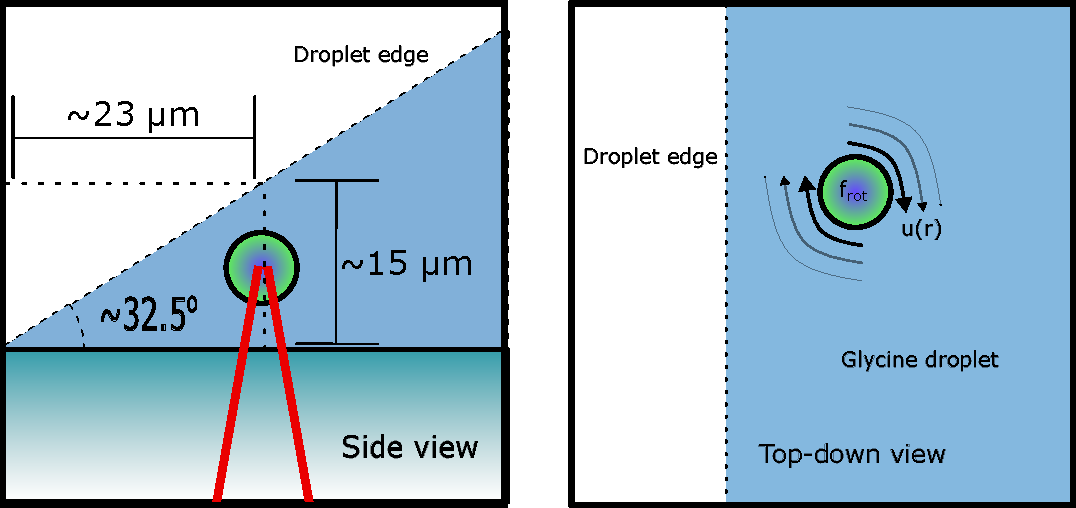
\includegraphics[width=\linewidth]{vaterite_diagram.pdf}
	\caption{Diagram of optical trapping set up for rotating 
		birefringent particles in a supersaturated solution. 
		Left: side view of the trapping set up showing the 
		location of the trap focus at the edge of the droplet 
		of a supersaturated solution. The approximate contact 
		angle (calculated by \cite{Flannigan2023}) is used to 
		provide a scale of how close a trapped particle could 
		be located. Right: top down view of the glycine droplet 
		with a trapped birefringent particle shown close to 
		edge of the trap. As the particle rotates the drag 
		force from the surrounding fluid generates a flow field 
		around itself (see Eq.~\ref{eq:birefringent_speed}).}
	\label{fig:3.9}
\end{figure}

Supersaturated solutions of glycine and water were prepared 
and stored in an incubator at $40^\circ C$ prior to use. 
When ready to be studied $15\ \mu L$ of vaterite suspension 
was pipetted into the solution and $20\ \mu L$ of the combined 
solution was pipetted onto the cover slip. A Vaterite sphere 
was located, trapped, and moved to the droplet edge where the 
solution meets the cover slip. This removed the need for 
hydrophilic coatings to achieve a flat fluid layer (as used by 
\cite{Liao2022, Rungsimanon2010}). 

Particle sizing was achieved by converting the particle diameter 
from pixels to physical units within an accuracy of $\pm0.05\mu 
m$. The QPD was used to measure the frequency of fluctuations 
in the QPD signal. After measuring the rotational frequency the 
sphere was left to rotate for a period of ten minutes after which, 
if no nucleation event was observed the particle was released. 
The overall results are catalogued in table~\ref{tab:Nucleation}.
\begin{table}[h!]
	\centering
	\caption{Results from rotating Vaterite within supersaturated solution of $H_2O$ and Glycine. Solubility concentration for Glycine at $16^\circ$ was $C^*=0.2016g/g$}
	\label{tab:Nucleation}
	\begin{tabular}[width=\textwidth]{|c|c|c|c|}
		\hline
		Super Saturation & Particle radius [$\mu m$] & $\omega$ [Hz] & Nucleation [$\checkmark/\times$]\\
		\hline
		\multirow{3}*{1.01} & 2.34 & 10.4 & $\times$ \\
		\cline{2-4} & 3.26 & 8.46 & $\times$ \\
		\cline{2-4} & 5.67 & 9.63 & $\times$ \\
		\hline
		\multirow{3}*{1.14} & 1.89 & 1.23 & $\times$ \\
		\cline{2-4} & 3.75 & 3.54 & $\times$ \\
		\cline{2-4} & 4.35 & 4.86 & $\times$ \\
		\hline
		\multirow{3}*{1.4} & 1.59 & 0.00 & $\times$ \\
		\cline{2-4} & 3.47 & 0.00 & $\times$ \\
		\cline{2-4} & 6.24 & 0.00 & $\times$ \\
		\hline
		\multirow{3}*{1.45} & 3.68 & 0.00 & $\times$ \\
		\cline{2-4} & 5.43 & 0.00 & $\times$ \\
		\cline{2-4} & 6.32 & 0.00 & $\times$ \\
		\hline
		\multirow{3}*{1.49} & 1.52 & $0.00$ & $\times$ \\
		\cline{2-4} & 4.76 & $0.00$ & $\times$ \\
		\cline{2-4} & 7.27 & $0.00$ & $\times$ \\
		\hline
	\end{tabular}
\end{table}

It should be noted that rotational frequencies equal to 
$0.00\ Hz$ are not due to a rounding error. Simply looking
at the live video shows no rotation of the vaterite particles,
and even looking at the QPD signals shows no discernable 
fluctuations that would arise due to rotation. Trying to trap 
a particle close to the edge proved more challenging than 
expected. Unlike in previous reports where the beam is 
focused at the upper edge of the droplet \cite{Liao2022, 
Yuyama2010, Sugiyama2022}, we attempted trapping in close 
to the contact point of the droplet and the cover slip. 

It is suspected that trapping is much harder at the 
interface due to increased surface tension and unpredictable 
scattering forces. The closest we could trap a microsphere to 
the droplet edge was in the range of $5-10\mu\ m$, at that 
distance the fluid flow is so low that even the presence of a 
hard boundary would be insufficient for shearing the fluid. 
Furthermore, as is evident in Table~\ref{tab:Nucleation}, 
the rotation rate drops off significantly with increased 
supersaturation, due to higher fluid viscosities. While in 
theory a sufficiently focused laser could rotate any 
microsphere to a fast enough to reach the shear rate 
predicted by \cite{Debuysschere2023} the localised intensity 
would be so large that even using $D_2O$ would see a significant 
increase in temperature. 

It is not impossible that fluid shearing could be used in the 
future to localise nucleation; but from these results, using 
individual micro-rotors is not an appropriate method due to
two key factors. Firstly, the area of influence is far too 
small to see any noticeable increase in the nucleation rate 
this is demonstrated most clearly in fig.~\ref{fig:vaterite_shear}. 
Due to the exponential decay in the expected shear rate it is 
very difficult trying to shear a large volume of fluid. Even 
if the optimal shear rate at a micro-level was an order of 
magnitude less than what was predicted by \cite{Debuysschere2023}, 
only a small volume of fluid would even experience that shear 
rate. In order to properly understand the microscopic effects 
of fluid shear a method of localised shearing over a larger 
fluid volume is necessary.  

Secondly, increased fluid viscosity significantly reduces 
the limits the maximum rotation rate possible. As indicated 
by \ref{tab:Nucleation}, the rotation rate achievable by a
vaterite sphere falls off significantly with increasing 
supersaturation. Experimental estimations of relative viscosities
showed a 12\% increase when looking at undersaturated glycine
solutions ($S\approx0.34$) \cite{Patyar2020}. As far as we
are aware there are no reported fluid viscosities for higher
supersaturations. Extrapolating the results from \cite{Patyar2020}
suggests that a saturated solution would have a 35\% increase 
in fluid viscosity (compared to pure water). This also does 
not account for any other factors such as the fact that close
to a boundary a rotating particle will experience a reaction
torque from the stationary surface \cite{Bruce2020}. 

If multiple micro-rotors could be trapped in close proximity 
to one another they could create a large region of fluid where 
nucleation is more likely than the bulk fluid. Because optical
torque is not contingent on the fluid properties the only 
limiting factor would be the total angular momentum transferred 
to each particle. Micro-rotors have been created that allow for 
precise control of suspended micro-particles \cite{Butaite2019} 
and could potentially be used to generate sufficient shearing. 
However these could not be used in this project as we lacked the 
necessary hardware to form multiple gradient traps.  
%%%%%%%%%%%%%%%%%%%%%%%%%%%%%%%%%%%%%%%%%%%%%%%%%%%%%%%%%%%%%%%%%%%%%%%%%%%%%
%%%%%%%%%%%%%%%%%%%%%%%%%%%%%%%%%%%%%%%%%%%%%%%%%%%%%%%%%%%%%%%%%%%%%%%%%%%%%
\section{Nucleation with a Stationary and Moving Beam}
As mentioned previously, shearing via optical rotation did 
not result in any localised nucleation events even while 
in the proximity of the droplet edge. An alternative approach
was suggested, using a galvano mirror to move a particle 
quickly through a supersaturated solution. Preliminary 
calculations suggested a particle moving rapidly through 
a fluid could produce significantly greater shear rates 
(see \emph{Appendix X.X} for breakdown) than a rotating 
particle. While a particle is within the optical trap the 
gradient forces are significantly reduced meaning simply 
trapping a particle is insufficient for inducing nucleation \cite{Flannigan2023}. This is why we did not see any 
nucleation events while rotating the vaterite, there is 
not a large gradient force to draw in material. 

During initial testing using silica beads we found that 
even in undersaturated solutions the optical trap would 
produce a crystal nucleus when the trap was empty. This 
has been reported prior \cite{Rungsimanon2010, Liao2022}, 
but what is more interesting is how the beam's motion 
influenced the growth of the nucleus. 

\subsubsection{Choice of Crystal growth rate units}
The growth rate of a crystal can be described using different
units depending on the situation. For example, seed crystals 
often use growth units in the form of \textit{length per unit
time}. This can either be used to describe the overall length
of the longest edge of a crystal, or to describe how individual
faces grow separately. This works well for crystals with a 
clear morphology, in regards to laser induced nucleation the 
crystal growth is heavily influenced by the local fluid 
conditions meaning tracking the length of an individual face 
is challenging. Instead we utilise image analysis software 
such as imageJ to measure the area of the crystal after each 
frame to get a rough estimate of the crystal growth rate in 
units of \textit{length$^2$ per unit time}. With the addition 
of the contact angle information from \cite{Flannigan2023} we 
can approximate the crystal height based on how close it is to 
the droplet edge.

\subsection{Stationary beam}
\label{sec:stationary}
Its well known that a supersaturated solution can nucleate
if irradiated by a focused beam with sufficient power 
\cite{Rungsimanon2010}. First we look at how a laser induced
nucleation event unfolds using a stationary focused beam. 
The laser was focused at the edge of a $20\mu L$ droplet 
consisting of water and dissolved glycine ($S=1.03$). The 
solution was monitored for 10 minutes, if a nucleation event 
was observed the event was recorded using a high speed CCD. 
If no nucleation event was observed after 10 minutes the 
solution was disposed of and a new sample was prepared. After 
ten repeats only 30\% of the samples observed a nucleation 
event at the focus. All of which displayed similar growth 
behaviour to one another.

Consider Fig.~\ref{fig:stationary_beam}, the frames taken from 
a nucleation event, the beam is a stationary being $\approx3.5 
\mu m$ from the droplet edge. After a period of roughly 5 minutes 
a nucleus forms at the trap focus, growing quickly (growth rate 
was approximated using imageJ to be on the order of $700\ \mu 
m^2/min$) from the focal point of the trap until after roughly 
$6$ seconds the crystal escapes. A likely reason that the trap 
is escaped is due to the fact that crystal is far too large to 
be held in place and is in fact still growing as the solution is supersaturated. Based on the contact angle measurements from \cite{Flannigan2023}, the droplet height could not have been 
any more than $2-5\mu m$ at the trap focus.
\begin{figure}[h!]
	\centering
	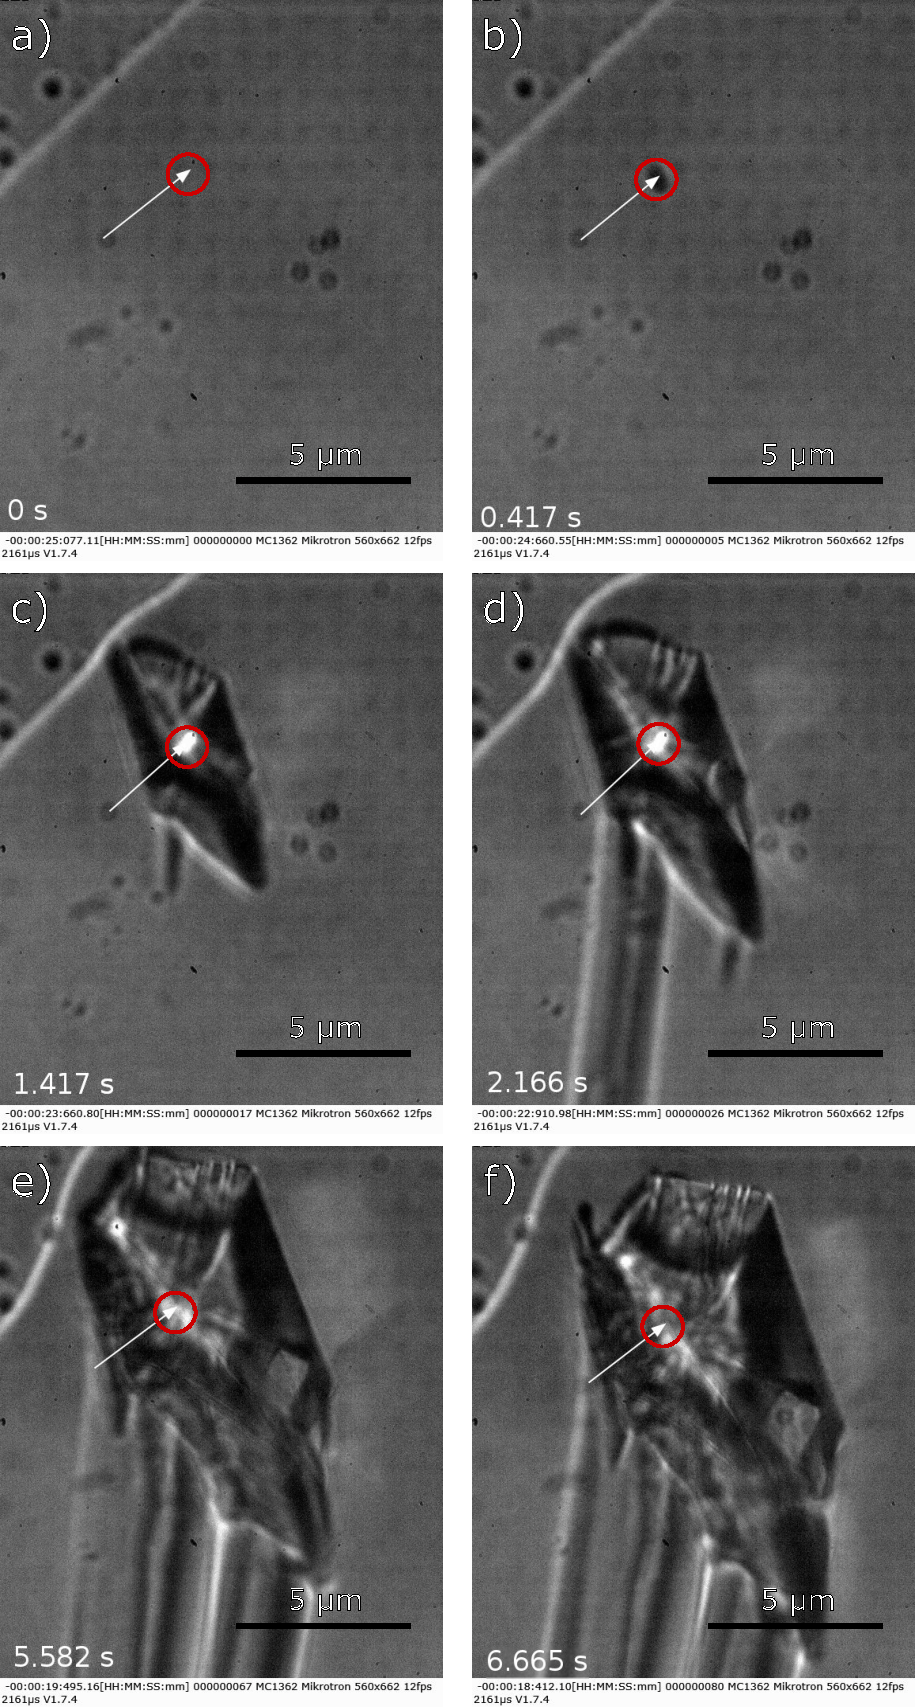
\includegraphics[width=\linewidth, height=1.3\linewidth]{frames_no_beam_movement.pdf}
	\caption{Laser induced nucleation at the edge of a droplet of supersaturated 
	glycine solution. (b) shows the first instance of a crystal nucleus, growing 
	quickly through (c)-(e) until after $6.665\ s$ the crystal begins to escape 
	the trap.}
	\label{fig:stationary_beam}
\end{figure}

Comparing to previous literature using optical tweezers shows 
that the growth rate is only loosely connected to the solutions 
supersaturation. Crystal growth rates for a solution of glycine 
and water ($S\approx1.00$) was found to vary from as much as 
$3900 \mu\ m^2/min$ to as low as $675\mu m^2/min$ 
\cite{Flannigan2023}. The reason for such high crystal growth 
rates is due primarily to the tweezer focus bringing in material 
due to gradient forces. A study of glycine crystals in water 
found that for a similarly supersaturated solution the growth 
rate along the {011} face was around $0.1\ \mu m/min$ where as 
the {010} face was found to have a growth rate of around $0.01\ 
\mu m/min$. While its difficult to extrapolate an exact area 
growth rate from these results we can approximate that if the 
we looked directly perpendicular to the crystal growth the area 
would increase at $\approx0.02\ \mu^2/min$ (see X.X for a 
breakdown of this approximation). 

The key take away to remember is that the beam has no influence 
over the crystal shape, instead it grows outward from the trap 
focus. Furthermore, due to the fact that the solution is 
supersaturated the crystal growth cannot be contained to the 
trap focus. Instead the crystal escapes as its size exceeds the 
trap focus. 

\subsection{Moving Beam}
\label{sec:moving}
To test if a rapidly moving silica bead could generate the 
necessary shear rate for crystal nucleation we wanted to 
see if a trapped silica bead could be trapped and moved in 
an aqueous solution. $20\ \mu L$ of glycine and water ($S=
1.03$) was added to $10\ \mu L$ of a dilute water-silica 
mixture making the solution unsaturated ($S\approx0.7$). 
However, due to the beam's motion we instead encountered 
unexpected growth behaviour. 

Shown below in Fig.~\ref{fig:eliptical_beam_1} where 
we have the laser focus moving in a small elliptical 
pattern. While nothing is seen directly entering the 
focus a nucleus forms close to the droplet edge, 
unlike in fig.~\ref{fig:stationary_beam} the crystal 
does not grow out from the focal point evenly. Due to 
the galvano mirror, the crystal is simultaneously 
being moved by and growing around the focal point of 
the trap. Because of this the crystal nucleus lacks 
a clear morphology at first. Until roughly $20\ s$ 
the crystal reaches a almost prismatic structure, 
with further irradiation increasing the size.
\begin{figure}[h!]
	\centering
	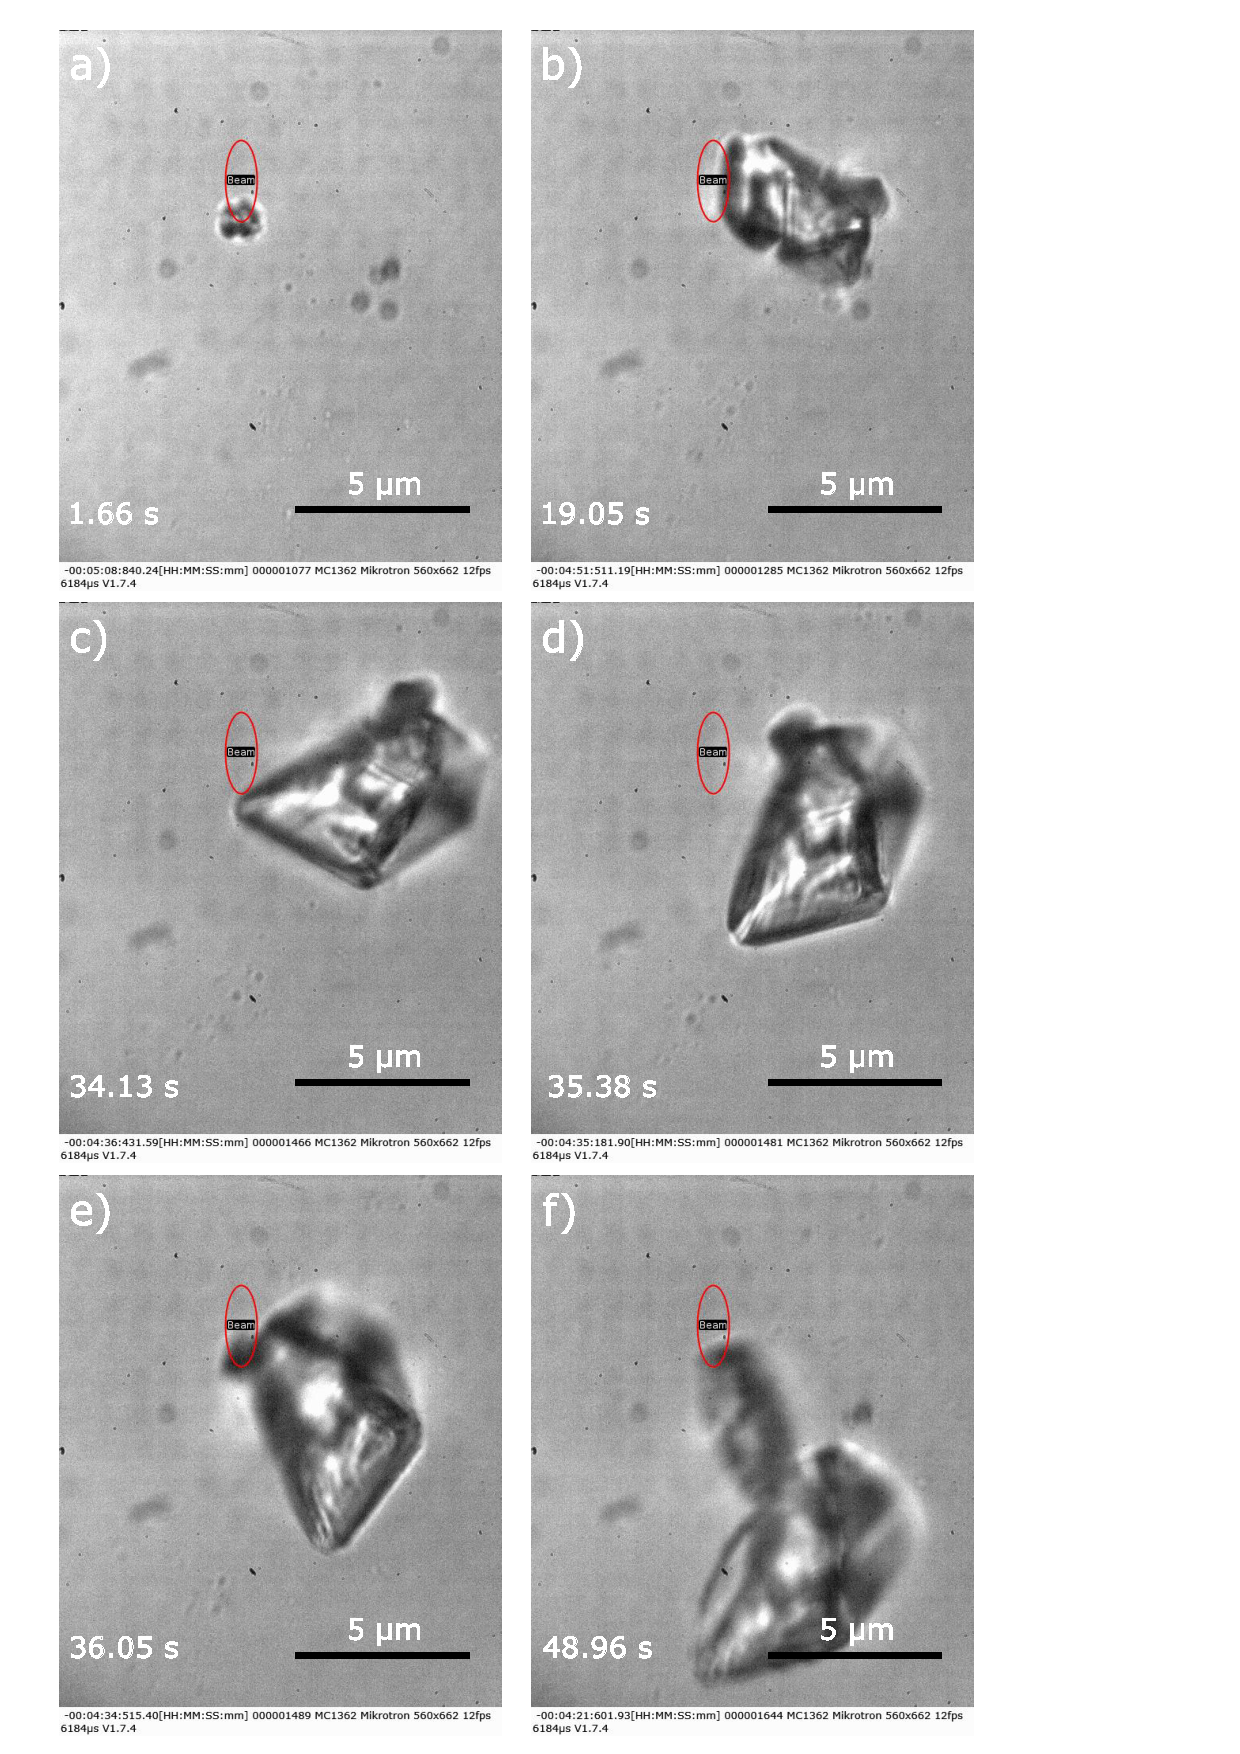
\includegraphics[width=0.8\linewidth]{frames_eliptical_beam.pdf}
	\caption{Frames from a longer video depicting the growth 
		of a nucleus using a moving beam. Beam power is kept 
		at 700 mW and the supersaturation was estimated at 
		S=0.86. Initially the crystal shape is amorphous (a) 
		but eventually reaches a more regular shape (b). This crystal is still influenced by the optical trap as 
		even when not directly irradiated by the laser the 
		crystal rotates between (c) and (d). When the laser 
		is focused on a corner the crystal growth is localised 
		to that region, resulting in an elongated section 
		forming between frames (e) and (f).}
	\label{fig:eliptical_beam_1}
\end{figure} 

Interestingly the galvano-mirror allows the trap to 
impart a slight torque on the crystal, as shown in fig.~\ref{fig:eliptical_beam_1}(c) and (d), where even 
though the crystal is not directly in the trap focus 
it rotates in the $x-y$ plane and gets trapped again 
at a corner. The rotation could not be due to fluid 
flow close to the surface of the crystal as the 
dipole moment of individual water molecules is too 
small to be influenced by an optical trap. In figs.\ref{fig:eliptical_beam_1}(e) and (f), the 
crystal growth becomes localised to the corner. The 
area growth rate between figures \ref{fig:eliptical_beam_1}
(a) and (d) was approximated using imageJ at $45.03\ 
\mu m^2 /min$, where as between figures 
\ref{fig:eliptical_beam_1}(e) and (f) the growth rate 
at that particular edge was estimated at $42.10\ \mu m^2/min$. 
 
Nucleation in undersaturated conditions has been 
reported previously in $D_2O$ \cite{Rungsimanon2010} 
and $H_2O$ \cite{Flannigan2023}, though not involving 
a moving beam. This modification allows for the crystal 
growth to be localised to a specific region of the bulk 
crystal whereas with a stationary beam there is no 
control over the crystal morphology. In fact this allows 
for a much finer control over the exact shape of the 
crystal nucleus, in some cases allowing for growth out
of the viewing plane as shown in fig.~\ref{fig:out_of_plane}.
\begin{figure}[h!]
	\centering
	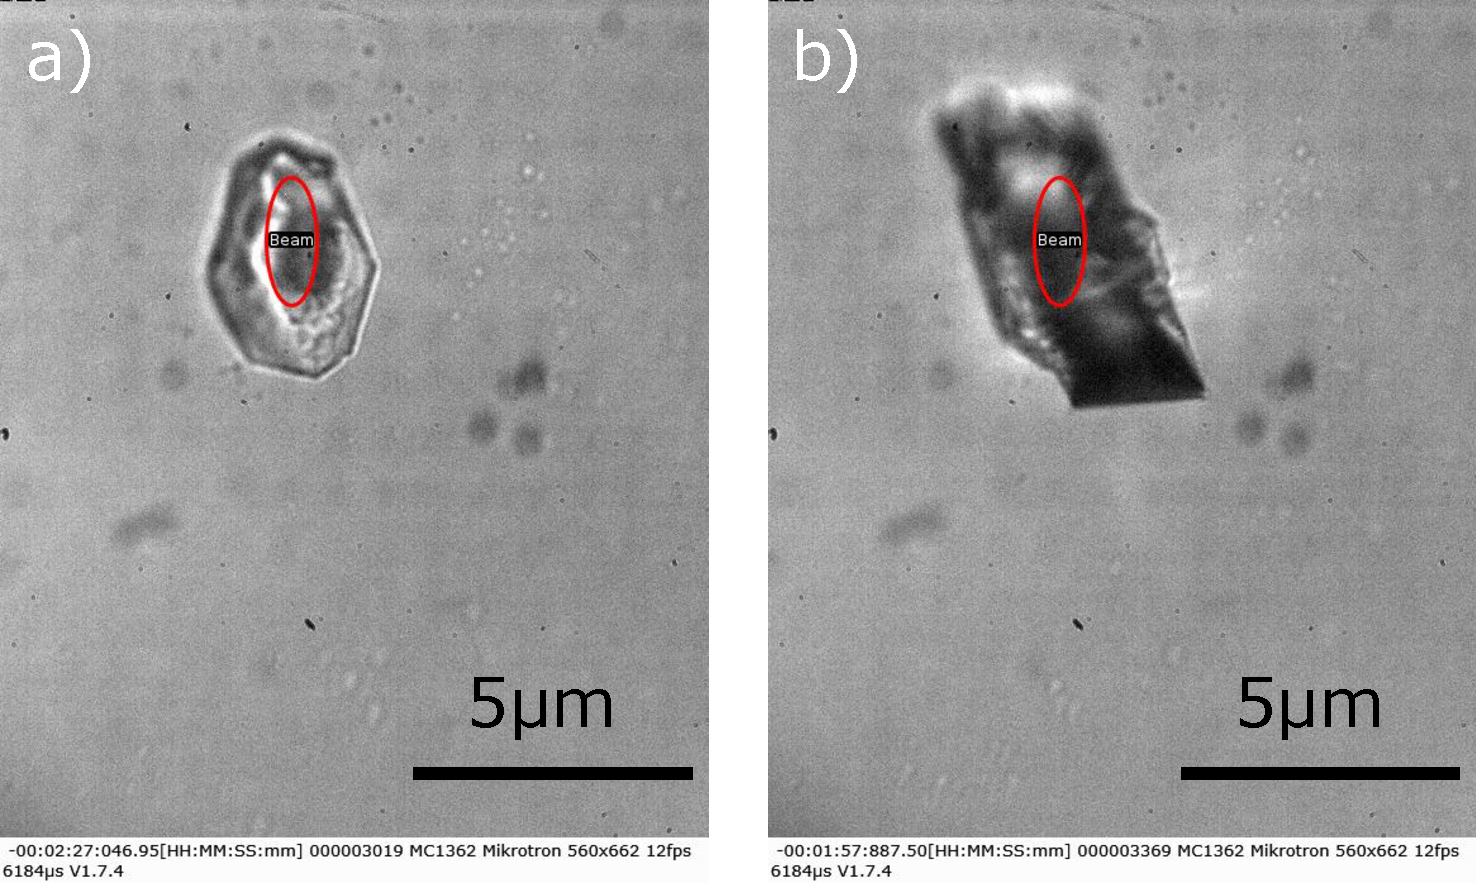
\includegraphics[width=\linewidth]{out_of_plane.pdf}
	\caption{Interesting crystal growth on the surface of an
	existing crystal. Initially the crystal surface seems 
	flat (a) but eventually a different crystal structure 
	grows out off of the surface (b).}
	\label{fig:out_of_plane}
\end{figure}

Where a large outgrowth forms on the surface of a nucleus,
over a period of $30\ s$ the outgrowth develops into a 
rhombic crystal structure. The unique crystal growth 
demonstrated is likely a factor of the moving beam focus,
but this raises a question over how the laser can localise
the growth only around the focus and why the crystal does 
not grow or shrink when not directly within the trap. There
should be some material that is being drawn into the trap
as it scans across the camera frame.

\subsection{Direct trapping of Glycine clusters}
\label{sec:clusters}
In a repeat experiment a solution similar to sec.~
\ref{sec:stationary} was made up, but without any 
silica micro-spheres. Once again the beam was focused 
close to the droplet edge, this time the galvano 
mirror was scanning a circular path (as shown in fig.~\ref{fig:cluster_trapping}). After a few 
minutes of irradiation droplets were seen entering 
the camera frame. Because no silica had been added, 
and that the solutions were filtered, these droplets 
had to be from the glycine solution. Trapping 
individual droplets did not result in immediate 
nucleation even after several minutes being trapped. 
Trying to bring two droplets together resulted in 
nucleation between the two droplets, compared to 
\ref{sec:stationary} \& \ref{sec:moving} the growth 
is much slower, taking nearly 40 seconds before the 
crystal structure becomes clearer.
\begin{figure}[h!]
	\centering
	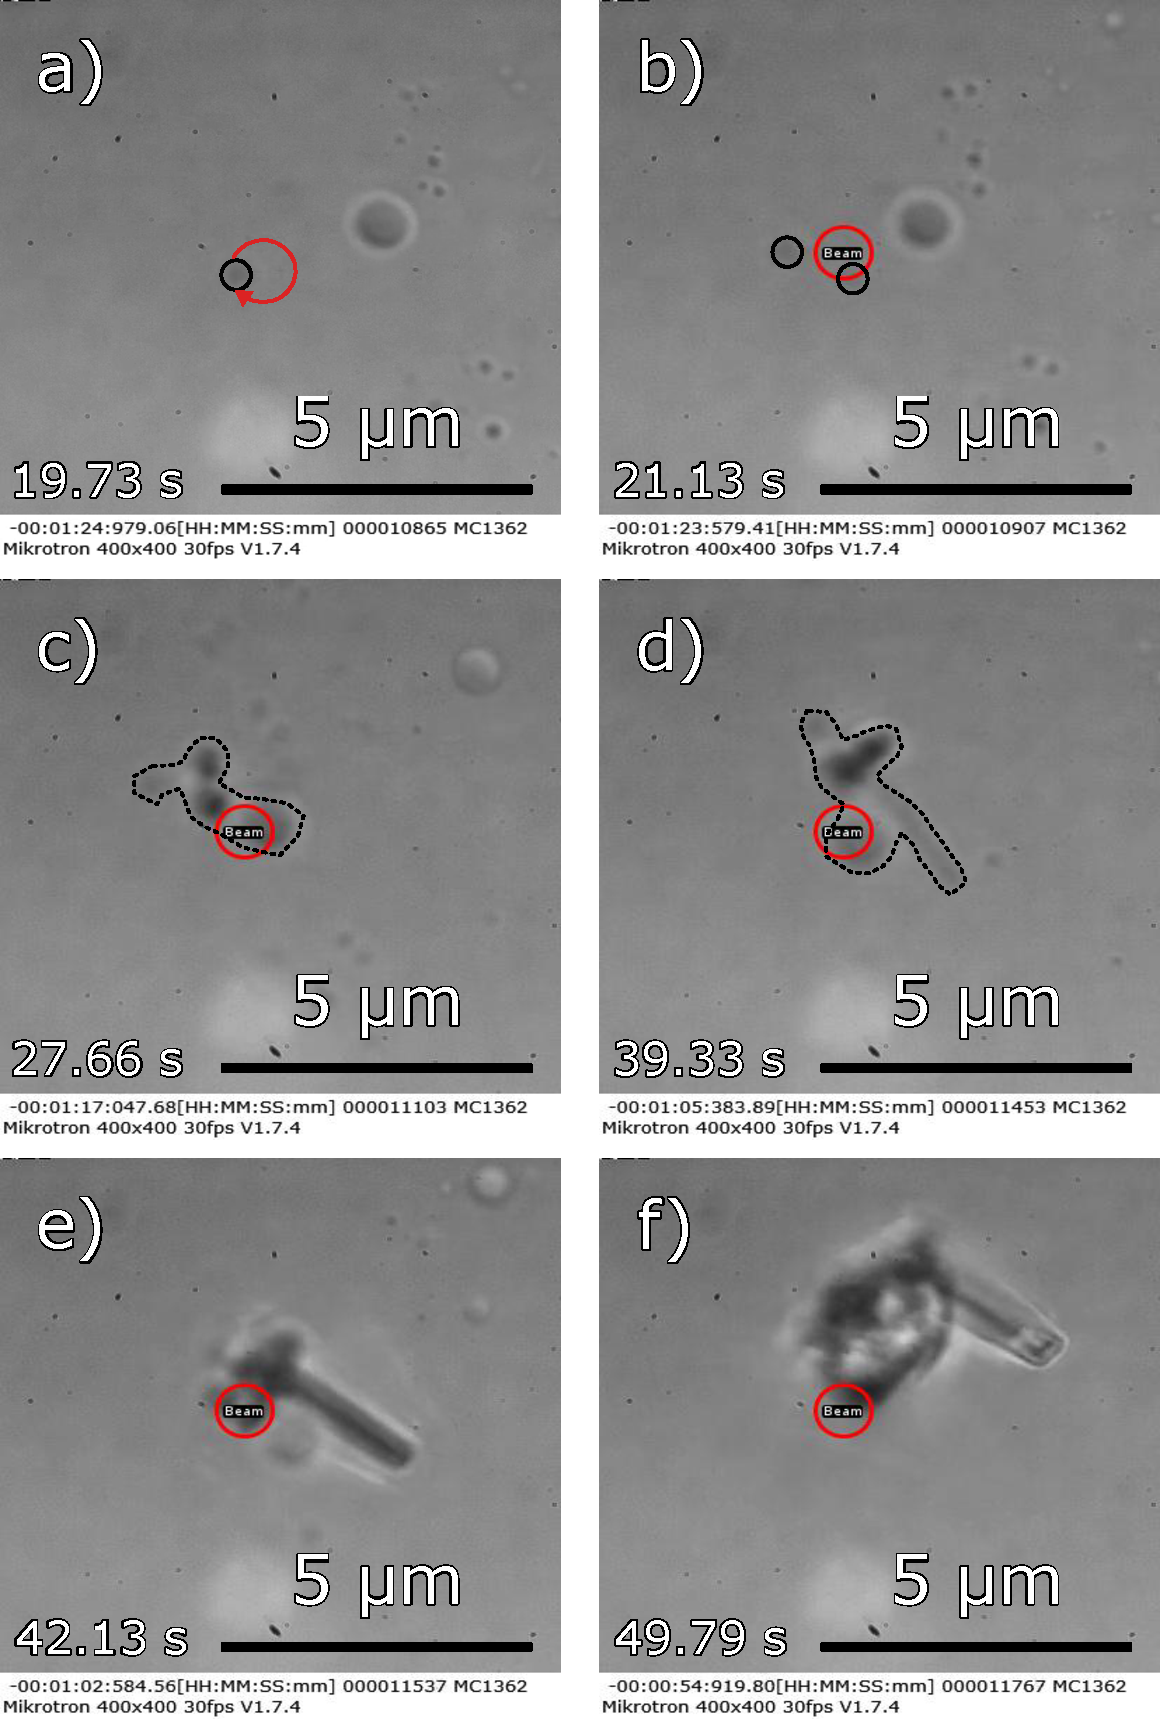
\includegraphics[width=0.8\linewidth]{cluster_trapping.pdf}
	\caption{Frames from a longer video demonstrating the trapping 
		of a glycine droplet. Solution is undersaturated glycine 
		and water (S = 0.86), with the laser power is set at $750\ 
		mW$. (a) shows a trapped droplet (outlined in black) being 
		brought into contact with a larger droplet. (b) upon contact 
		a nucleus can be seen between the two droplets. The growth 
		is rather slow with the crystal having no clear defined 
		morphology through (c) and (d). Between frames (e) and (f) 
		the larger droplet finally joins the main crystal.}
	\label{fig:cluster_trapping}
\end{figure}

The fact that these droplets can be trapped indicates 
they must have a higher refractive index than the 
surrounding solution. Previous reports have shown that 
a focused trap will draw in solute material from the 
bulk \cite{Tsuboi2009, Gowayed2021}. This suggests that 
the droplets observed are concentrated spheres of glycine, 
which also explains how nucleation was initiated when those
two spheres were brought into contact with one another. The 
droplets must be providing material for the crystal growth.
It has been shown that the concentration of glycine solution 
is correlated with the refractive indices of the liquid 
\cite{Gowayed2021, Orttung1963}. This suggests that we could
measure the concentration of individual droplets based on the
trapping strength of each droplet. 
\newpage

\subsection{Influence of a moving beam front on seed crystals}
\label{sec:seed_crystals}
One potential application of this phenomena would be in using 
a moving the moving beam front as a method for shaping the 
final crystal morphology. Therefore, we wanted to test if a 
moving beam front could have any influence on the shape of a
seed crystal submerged in a bulk solution. Glycine seed crystals 
were grown via evaporative crystallisation over night. The 
resultant crystals were as wide as $0.5 mm$ in some cases. 
Individual crystals were collected and suspended in a water 
+ glycine solution ($S = 1.001$) and the laser was scanned 
along a narrow linear path. It should be noted that the seed 
crystal was fully submerged in the solution, meaning that there
is no interface between the air and solution close to the seed.
Five separate repeats were conducted, all demonstrating similar
behaviour to one another.  

As shown by fig.~\ref{fig:seed_crystals} the laser does not 
in fact promote crystal growth but instead forces the crystal 
to dissolve into the bulk solution. The dissolution rate is not 
as substantial as the growth rate seen in previous sections. 
It takes over 20 minutes for the for the crystal surface to 
dissolve more than a few microns. Furthermore we do not report 
any sightings of droplets close to the surface of the crystal 
nor do we see anything enter the optical trap.
\begin{figure}[h!]
	\centering
	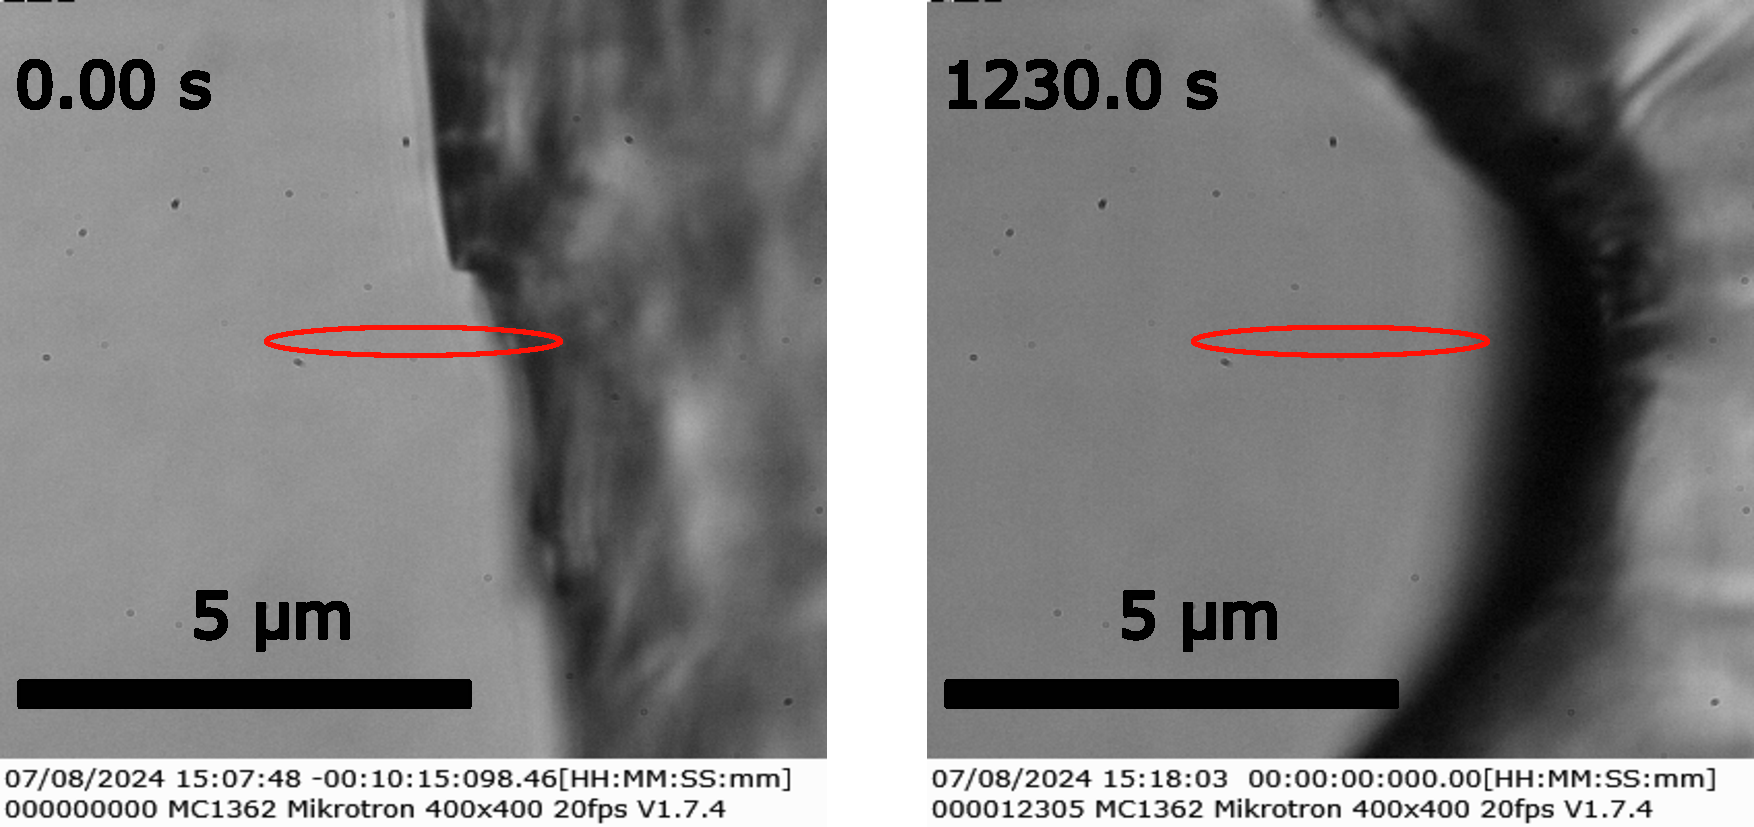
\includegraphics[width=\linewidth]{seed_crystals.pdf}
	\caption{Frames from a seed crystal being irradiated by a 
		scanning laser. The laser path is shown below in red. 
		Initially the crystal edge is nearly perpendicular to 
		the laser path. Over the course of nearly twenty minutes 
		the crystal around the laser has dissolved leaving a 
		concave indent.}
	\label{fig:seed_crystals}
\end{figure}

This has some implications: Firstly, the lack of supposed 
glycine droplets suggests that the presence of an interface 
is crucial in order to promote the formation of these droplets. 
This is consistent with previous reports on laser nucleation, 
where a air-solution or solution-glass interface is necessary 
for the trap focus to have any noticeable effect on the solute \cite{Gowayed2021, Liao2022, Rungsimanon2010}. Secondly, the 
fact that the seed crystal dissolved in a saturated solution 
suggests that this could be due to a localised heating effect. 
A commonly used heating model for optical tweezers is the 
Peterman model \cite{Peterman2003} which accounts for the lateral 
distance between the optical trap and a local heat sink (such 
as the glass cover slip or microscope objective). Even with 
the heat sink the predicted temperature rise in pure water would 
be around $5-10 K$.  The fact that the seed crystal dissolves 
so slowly could simply be due to the fact that the local heating 
is lessened by the moving beam front.
 
\section{Summary of Moving Beam Phenomena}
To summarise, the introduction of a moving beam helps to 
accelerate the local growth of a newly formed crystal. It 
seems that this phenomena will only occur when close to 
interface between the solution and air. We note the presence
of droplets that can sometimes be seen entering the trap, 
though this is not always necessary for a nucleation event 
to occur. A plausible description of the phenomena is described
thusly. 

Initial nucleation is similar to typical optical trapping 
induced nucleation, with the air solution interface limiting 
the molecular mobility of the solute molecules \cite{Liao2022, 
Sugiyama2009, Gowayed2021}. The moving beam front can influence 
the motion of the nucleus initially, but eventually the drag 
force means the crystal is not moved by the optical trap. 
Localised crystal growth occurs when the trap is close to or 
partially over the interface of the crystal (see fig.~
\ref{fig:local_nucleation}(a)). This suggests that the 
laser itself is bringing in new solute material that can then
adhere to the crystal surface. Interestingly even when the 
crystal growth is localised to a small section of the crystal
we do not observe the crystal dissolving. This is consistent 
with other observed laser induced nucleation results, where 
as long as the laser is active the crystal remains stable 
within the solution \cite{Flannigan2023, Rungsimanon2010,
Liao2022, Sugiyama2009}. It does raise further questions 
however, mainly in an undersaturated solution is a moving 
beam front able to increase the size of the formed nucleus
compared to a stationary beam? Additionally, it raises the 
question about what the role the 'glycine droplets' play in 
the nucleation process.

As shown in \ref{sec:clusters}, the optical trap can manipulate 
these droplets similar to microspheres. When in close proximity 
to the trap these droplets are brought towards the crystal 
surface (see fig.~\ref{fig:local_nucleation}(b)). We have 
already suggested that these droplets must contain glycine as 
they are to large to be a silica microsphere, and the solutions 
were filtered prior to being studied. The droplets provide 
material that grows the crystal around that region (see fig.~\ref{fig:local_nucleation}(c)). Eventually the local 
solution is either depleted of solute material or the crystal 
front has grown to fully encompass the trap, preventing further 
growth (see fig.~\ref{fig:local_nucleation}(d)). 
\begin{figure}[h!]
	\centering
	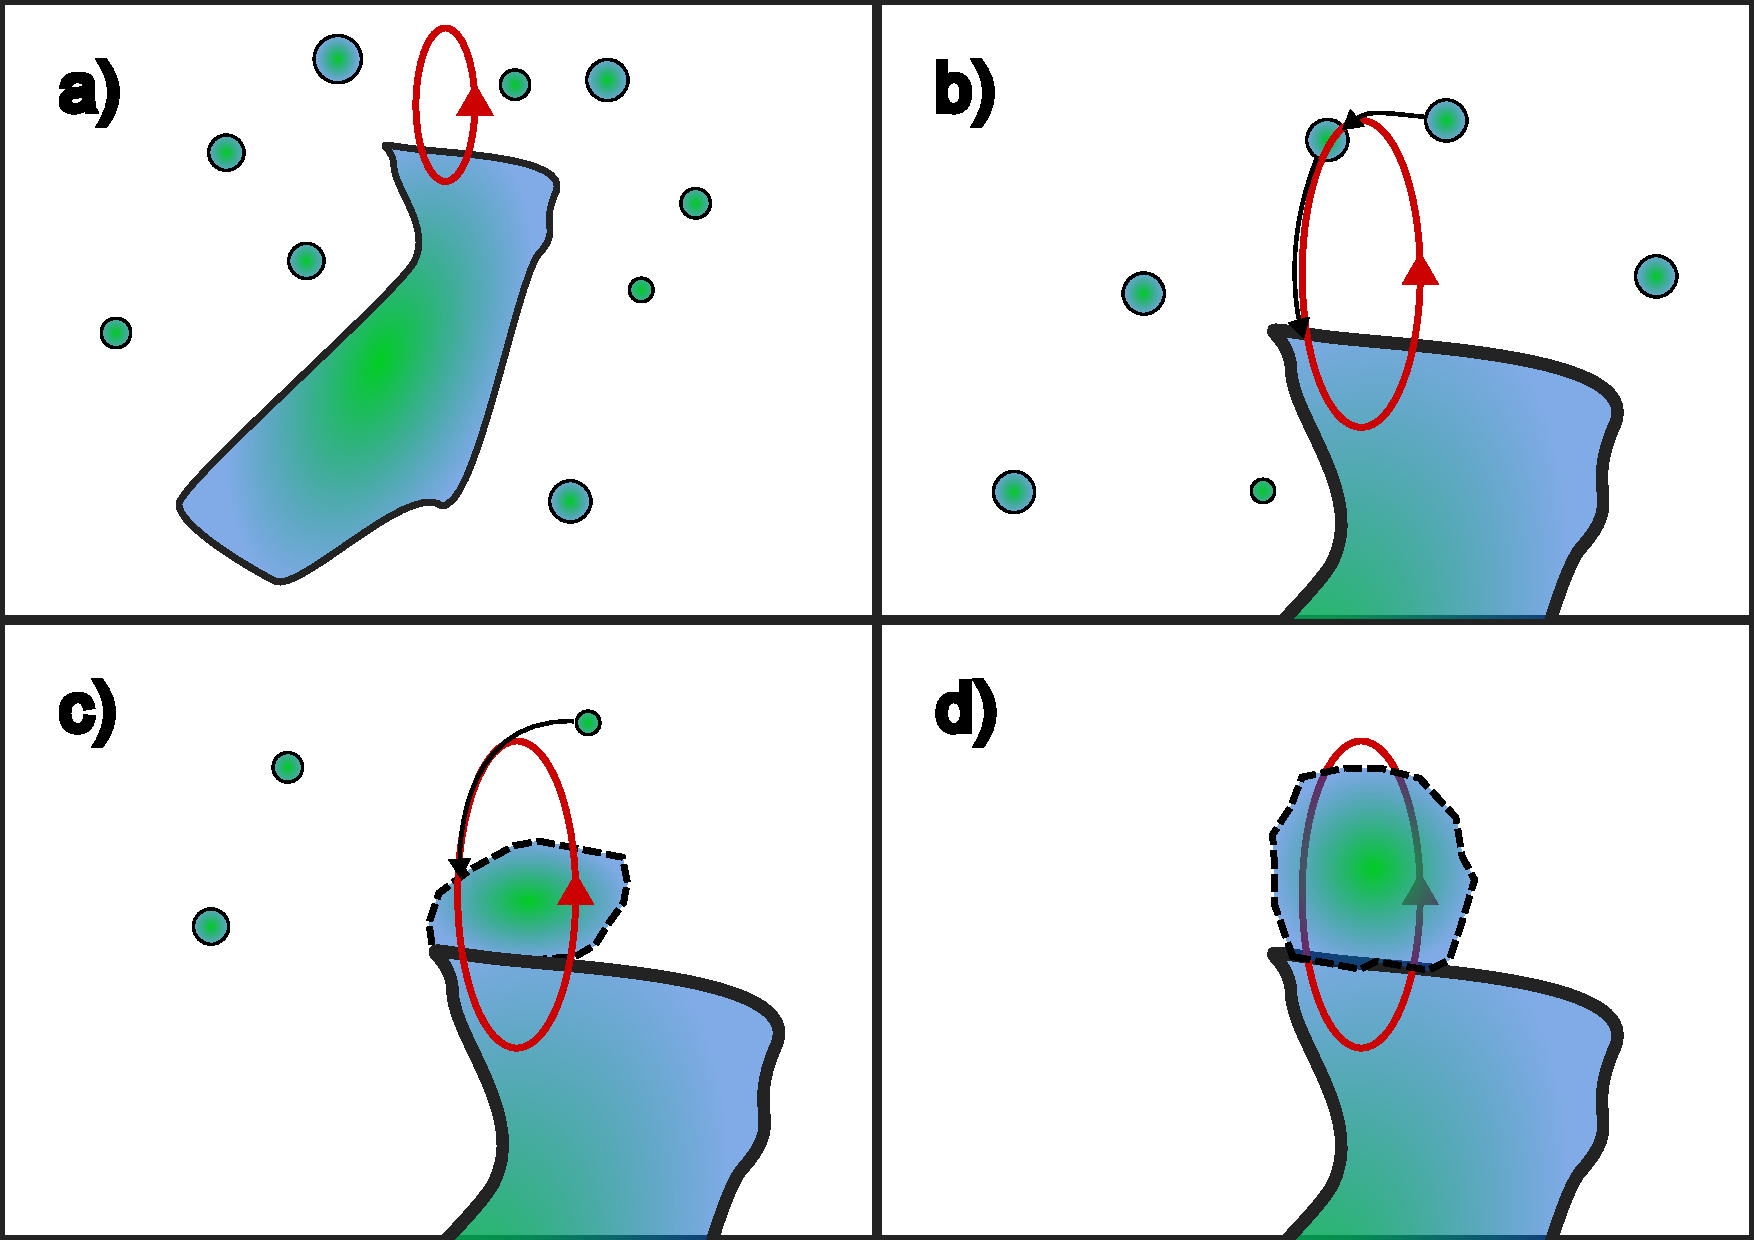
\includegraphics[width=0.8\linewidth]{galvano_diagram.pdf}
	\caption{Diagram outlining how a moving beam assists in the 
		growth of a crystal nucleus. (a) a crystal nucleus is 
		partially trapped by a moving beam with solute droplets 
		close to its surface. (b) droplets close to the laser
		focus can be drawn in by gradient forces and moved 
		towards the crystal surface. (c) the laser brings in 
		material that is then deposited on the surface of the 
		crystal. (d) eventually the crystal area either fully 
		surrounds the laser focus or the solution surrounding 
		the laser is depleted of solute material.}
	\label{fig:local_nucleation}
\end{figure}

What remains unclear is why the solution interface is necessary
for localised crystal growth. We know that the glycine droplets 
will form when the laser is close to the glass-solution interface
\cite{Gowayed2021, Yuyama2010, Yuyama2012}. This is consistent 
with our results as being able to image the droplet edge requires 
that the laser is brought close to the cover slip. However it is 
not clear how exactly these droplets contribute to localised 
crystal growth as in sec.~\ref{sec:moving} no droplets are seen 
entering the trap. It seems likely that the presence of droplets 
is necessary as we see that the seed crystals dissolve while 
there are no droplets present. 

There are still several factors that need to be investigated. 
Firstly, there is the question of what conditions result in the 
production of concentrated droplets, it is not clear if the 
presence of a laser is required or if these droplets naturally 
occurring. Prior literature would suggest that the laser is 
required \cite{Liao2022, Tsuboi2009}, but this would not explain 
why in many cases the droplets are found far outside the influence 
of the optical trap. It has been shown that phase separation 
occurs when a trap is focused close to the cover slip 
\cite{Gowayed2021, Yuyama2010, Yuyama2012}, but there has been 
no cases of nucleation occurring at the cover slip. Furthermore
these experiments all occurred in supersaturated condition 
($S\ge 1.50$) with a much wider focus ($NA \le 1.00$) whereas 
our results occurred in undersaturated conditions with a 
tighter focus. We did not not any occurrence of a phase 
separation as reported by \cite{Gowayed2021, Yuyama2010, Yuyama2012}
and yet we see the appearance of droplets that we surmise 
are partially constructed of glycine.

Secondly, there is the question of how these droplets supply 
material to the bulk crystal. In some instances it is clear 
that the droplets are being drawn into the trap, however, in 
other instances while there are no droplets close to the 
vicinity of the optical trap the crystal continues to grow. 
If these droplets are a necessary precursor to induce crystal 
nucleation then understanding how they provide materials to 
the bulk crystal may help with our understanding of the 
kinetics of multi-step nucleation. 

\section{Conclusion}
In conclusion, the experimental results from this chapter 
provide no affirmative evidence of shear induced crystal 
nucleation. This is in part due to the limited rotational 
speed that could be achieved using vaterite microspheres. 
Simply adding a micro-rotor to a supersaturated solution 
will not yield a significant fluid flow to induce crystal 
nucleation. Furthermore, the region in which the local 
shear rate is significant enough is so small that any 
nucleation events that could occur there may not grow large 
enough to be stable. This does not however, suggest that 
shear induced nucleation is impossible at a micro scale. 
In fact there have been several developments lately that
allow for the precise rotation of multiple rotors to 
control the precise motion of silica beads \cite{Butaite2019}. 
This would allow for direct control of the shear rate 
within a given volume of fluid, allowing one to study the 
impact of fluid flow on a nucleus at a micro-scale.

On the other hand, the results utilising the galvano mirror 
have some interesting implications for future research into 
crystal nucleation using optical tweezers. We noted that a 
moving beam front is capable of localising the crystal growth
around the beam focus in undersaturated conditions. Typically
in laser induced nucleation the final crystal morphology is 
influenced primarily by the local fluid conditions 
\cite{Flannigan2023, Liao2022}. If this phenomena could be 
fully understood we could have a means of directly manipulating 
the morphology of any nucleating crystal. We noted that in 
undersaturated conditions the presence of droplets that could 
be trapped and later nucleated when brought into contact with 
one another. There remains some uncertainty over the role these 
droplets play in a nucleation event. Further research is also 
necessary to understand how the fluid and laser parameters 
(i.e. supersaturation and numerical aperture) impact the 
formation of these droplets. The fact that these droplets could 
be trapped suggests they have a higher refractive index to the 
solution, given that the solutions were filtered prior to 
irradiation dismisses that they could be dust particles. Prior 
literature suggests that optical trapping of a supersaturated 
solution can lead to the production of nano droplets 
\cite{Gowayed2021, Tsuboi2009}. 



\printbibliography
	
%%%%%%%%%%%%%%%%%%%%%%%%%%%%%%%%%%%%%%%%%%%%%%%%%%%%%%%%%%%%%%%%%%%%%%%%%%%%%%%%
%%%%%%%%%%%%%%%%%%%%%%%%%%%%%%%%%%%%%%%%%%%%%%%%%%%%%%%%%%%%%%%%%%%%%%%%%%%%%%%%
%%%%%%%%%%%%%%%%%%%%%%%%%%%%%%%%%%%%%%%%%%%%%%%%%%%%%%%%%%%%%%%%%%%%%%%%%%%%%%%%
\end{document}
